\documentclass[11pt,a4paper]{article}

\usepackage[UTF8,heading=true]{ctex}
\usepackage{amsmath,amssymb}
\usepackage{booktabs}
\usepackage{multirow}
\usepackage{geometry}
\usepackage{graphicx}
\usepackage{xcolor}
\usepackage[colorlinks=true,linkcolor=blue!55!black,citecolor=blue!55!black,urlcolor=blue!55!black]{hyperref}
\usepackage{enumitem}
\usepackage[authoryear,round]{natbib}
\bibliographystyle{apalike}
\usepackage{caption}
\captionsetup{font=small,labelfont=bf}
\geometry{left=2.4cm,right=2.4cm,top=2.5cm,bottom=2.5cm}
\setlength{\emergencystretch}{2.5em}

% ctex 会把「摘要」以及图表标题前缀本地化成中文（摘要 / 表 N / 图 N）。
% 本文是英文投稿，这几处必须是英文，否则每一条图表标题都以汉字开头。
\renewcommand{\abstractname}{Abstract}
\renewcommand{\tablename}{Table}
\renewcommand{\figurename}{Figure}
\renewcommand{\refname}{References}

\newcommand{\X}{\mathbf{X}}
\newcommand{\Xt}{\tilde{\mathbf{X}}}
\newcommand{\E}{\mathbb{E}}
\newcommand{\FDP}{\mathrm{FDP}}
\newcommand{\FDR}{\mathrm{FDR}}
\newcommand{\ld}{\lambda_{\min}}

\title{\bfseries A pre-analysis diagnostic for reference-cohort model-X
knockoffs in neuroimaging\\[6pt]
\large Feature geometry sets the ceiling; the number of true signals, cohort
mismatch and the penalty constant govern the outcome}

\author{%
  Jiale Li\thanks{Corresponding author. \texttt{240902057@njnu.edu.cn}} \and
  Siqin Zhang\thanks{\texttt{240902100@njnu.edu.cn}} \and
  Xinyue Jiang\thanks{\texttt{250901007@njnu.edu.cn}}%
  \\[4pt]
  \small School of Mathematical Sciences, Nanjing Normal University,
  Nanjing, China
}
\date{September 2026}

\begin{document}
\maketitle

\begin{abstract}
\noindent
Model-X knockoffs give finite-sample FDR control under an arbitrary response
model, but in neuroimaging the covariate distribution must be estimated from
a reference cohort, and the procedure often reports
nothing. We supply a diagnostic computable from the reference cohort before any
knockoff is drawn, and establish what it predicts.

The diagnostic is the effective rank of the ROI summary's covariance,
set by the summary, not the cohort. Averaging Fisher-$z$ connectivity
over all other parcels---the field's default---makes each feature a row mean
of a correlation matrix, hence a proxy for its first principal component:
median $R^2=0.677$, effective rank $2.56$ of $113$. Partial correlation gives
$71.6$, unregularised $59.8$. The four summaries agree at median $r\le0.26$,
every ROI below $0.5$.

Known-truth controls delimit this. A low effective rank does not
explain a null result: with the real
covariance the pipeline attains power $0.859$; reference-cohort size buys a few points of power,
not the outcome; what binds is the number of true signals ($0.97$ at $k=12$, $0.20$ at $k=3$). Six constructions
are indistinguishable; a mirror method keeps validity only by giving up power.

Validity is separate. Cohort mismatch of $0.12$--$0.19$ breaks FDP control
while \emph{raising} power; after subtracting a sampling-noise floor it is
negligible in ABIDE~I and II but $0.117$ in ADHD-200, whose FDP is exceeded. The penalty constant must satisfy power and convergence at once.

A cohort of another disorder replicates the ordering but not the severity:
the diagnostic generalises, the constants do not.
\end{abstract}

\noindent\textbf{Keywords:} model-X knockoffs $\cdot$ false discovery rate
$\cdot$ reference cohort $\cdot$ neuroimaging $\cdot$ effective rank
$\cdot$ reproducibility

\bigskip

\section{Introduction}
\label{sec:intro}

\paragraph{The problem.}
Identifying which of many measured quantities a phenotype depends on is
central to neuroimaging. A region-of-interest (ROI) study measures $p\sim
10^2$ features per subject and asks which are associated with a diagnosis or
a cognitive score. Testing each feature marginally inflates false
discoveries, and the conventional remedy---Benjamini--Hochberg on
$p$-values---presupposes valid $p$-values that, for the models practitioners
fit, either do not exist or are badly non-uniform in finite samples
\citep{dezeure2015high}. The arithmetic is unforgiving: brain-wide
association effect sizes are $r\approx0.01$--$0.05$, so reproducible
individual-level inference requires thousands of subjects
\citep{marek2022reproducible}, and cluster-based fMRI inference fails badly
enough to have been documented in detail \citep{eklund2016cluster}.

\paragraph{Model-X knockoffs.}
The knockoff filter \citep{barber2015controlling} sidesteps $p$-values.
Its original form assumes a homoscedastic linear model with $n\ge2p$; the
model-X extension \citep{candes2018panning} removes both restrictions. By
treating the covariates as random and assuming $F_X$ \emph{known}, it gives
exact finite-sample FDR control with no assumption on the response model and
no constraint on $p$ relative to $n$. Construct a synthetic copy $\Xt$ of
the covariates satisfying pairwise exchangeability and independent of the
response given $\X$; under the null the sign of the knockoff statistic is an
independent fair coin flip, so the number of large \emph{negative}
statistics estimates the number of false discoveries among the large
positive ones. The framework has been generalised to more efficient samplers
\citep{bates2021metropolized}, faster conditional randomisation
\citep{liu2022fast}, better constructions \citep{spector2022powerful}, and
sharper power theory \citep{wang2022power,liu2019esd,ke2024power}.

\paragraph{The price is $F_X$, and the received explanation for the bill.}
$F_X$ being known is the framework's entire cost, and in neuroimaging it
cannot be met: the covariate distribution must be estimated from an
independent reference cohort. That this substitution is not benign is known
on the validity side---FDR inflation is bounded by a divergence between true
and working conditional distributions \citep{barber2020robust}, exact control
survives estimated parametric families with $\Omega(n^*p)$ parameters
\citep{huang2020relaxing}, and asymptotic control holds under coupling
\citep{ark2025}, moment matching \citep{fan2026moments} or data splitting
\citep{fan2020rank}. It is also known on the practical side, in the adjacent
literature on genome-wide association, where knockoffs and fine-mapping
methods estimate linkage disequilibrium from an external reference panel and
where panel mismatch is a documented source of FDR inflation
\citep{benner2017finemap,chen2021ldref,kanai2022slalom}.

Knockoffs are now applied to ROI-level connectivity and to network
comparisons between groups \citep{ji2024differential}, and alternatives to
the equicorrelated construction are benchmarked on exactly this kind of data
\citep{chen2023systematic}. The explanation we examine here is the first one
those applications invite: the reference covariance is nearly singular, the
equicorrelated construction reads $\ld(\hat\Sigma)$ directly, and the
resulting knockoffs are too close to the originals to be distinguished from
them. That description of the spectrum is correct, and the construction
literature has addressed its consequences
\citep{spector2022powerful,candes2018panning}. Our question is whether it
explains the outcome.

\paragraph{What this paper does.}
We supply a diagnostic that a practitioner can compute from the reference
cohort alone, before any knockoff is drawn, and we establish what it predicts
and what it does not. The diagnostic is the effective rank of the ROI
summary's covariance. It predicts power; it does not predict validity, and we
give the two conditions that separately govern the latter. Arriving at it
required first testing the explanation the field reaches for---that the
reference covariance is too degenerate to build knockoffs from---and finding
that it fails; we report that rejection because it is the reason the
diagnostic points where it does. Figure~\ref{fig:flow} summarises the design
and fixes the scope of the claim. The argument has three moves.

\emph{First, the hypothesis fails its own test.} Three independent
manipulations of the covariance---using the real covariance as ground truth,
varying reference-cohort size from 100 subjects to none, and introducing the
distribution shift actually observed between ABIDE's cohorts---each fail to
reproduce the null result (\S\ref{sec:boundary}--\ref{sec:limits}). What
limits power in simulation is the number of true signals, a property of
knockoff$+$ itself.

\emph{Second, we exhaust the machinery.} We compare six knockoff
constructions, a mirror-based method that never inverts $\Sigma$, a
multi-environment filter that tests cross-site consistency, and a
one-parameter family of matrix-power transforms. None of them rescues the
outcome (\S\ref{sec:exhaust}--\ref{sec:matrixpower}), and we report for each
what the evidence actually supports---including the multi-environment filter,
which turns out to have too little power in this configuration to support any
conclusion, a fact its own positive control establishes. The matrix-power
family is worth singling out: it produces a continuous curve along which
the procedure's own reported error improves monotonically while its true
error degrades monotonically, and a global-null control confirms the
crossing.

\emph{Third, the feature geometry sets the ceiling.} Averaging
Fisher-$z$ connectivity over all other parcels---the field's default, global
brain connectivity \citep{cole2012global}---makes each feature a row mean of
a correlation matrix, and a row mean is a proxy for the first principal
component. In our data the median $R^2$ of a single feature on PC1 is
$0.677$ and the effective rank is $2.56$ of $113$. That the row sum of a
connectivity matrix is dominated by PC1 has been observed at the group level
\citep{vandenheuvel2025lnm} and for mean connectivity maps
\citep{moujaes2024ketamine}; we quantify it per subject, per feature, in a
variable-selection context, and show that it bounds what any downstream
method can achieve (\S\ref{sec:geometry}). It does not, however, set the
power: across the $41$ covariance configurations we sweep, spanning effective
rank $2.2$ to $113$, per-signal power never falls below $0.770$, whereas
changing the number of true signals moves it from $0.97$ to $0.20$.

We state at the outset what this paper is not. It is not a claim that
model-X knockoffs are invalid, nor that they cannot work in imaging. The
method is used here as designed, and it is the only framework in this
literature with a finite-sample guarantee to characterise. Our contribution
is to locate where that guarantee is achievable and where it is not, and to
supply a diagnostic---computable before any analysis is run, from the
reference cohort alone---that tells a practitioner which side of the
boundary they are on.

\section{Methods}
\label{sec:methods}

\subsection{Data}
\label{sec:data}

\textbf{ABIDE~I} \citep{dimartino2014autism} was obtained from the FCP-INDI
public archive in the \texttt{cpac/filt\_noglobal} branch (1{,}035 subjects,
20 sites), together with the \texttt{niak/filt\_noglobal} branch for the
pipeline comparison of \S\ref{sec:pipeline}. Subjects with
$\texttt{func\_mean\_fd}\ge0.2$ were excluded ($1{,}035\to885$; $14\%$).

We additionally observed \emph{constant} parcel time series---a signature of
incomplete brain coverage---in $68$ of $885$ subjects ($7.7\%$),
concentrated by site (CMU $80\%$, SBL $69\%$, CALTECH $46\%$, PITT $29\%$;
all others $\le5\%$) and by region ($60\%$ of affected parcels in the
inferior cerebellum and vermis). Such channels produce undefined
correlations; we mark them missing rather than imputing a value, remove
parcels missing in $>20$ subjects, then remove subjects incomplete on the
retained parcels. For AAL116 \citep{tzourio2002automated} this yields
$p=113$, $n=852$; the procedure was applied identically to Harvard--Oxford
and CC200 \citep{craddock2012whole}.

\textbf{ABIDE~II} \citep{dimartino2017abide2} was obtained from the same
archive (\texttt{Derivatives/DCAN}; Power2011 parcellation, CIFTI parcel time
series, $p=94$, $n=956$). The two cohorts share the disorder and almost
nothing else: different participants, scanners, sites, parcellation,
pipeline and file format.

\textbf{ADHD-200} \citep{bellec2017adhd200} is the third cohort and the
out-of-sample test of \S\ref{sec:shift} and \S\ref{sec:third}. It differs
from both ABIDE cohorts in disorder, participants, scanners, sites,
preprocessing pipeline and parcellation. We used the Athena-preprocessed
release with the AAL116 parcellation, retaining only runs whose distributed
quality flag is \texttt{1}: of $768$ subjects, $93$ failed and $11$ at the
three Peking sites are flagged as unevaluated, which we excluded
conservatively, leaving $n=664$ ($427$ controls, $237$ ADHD, nine sites;
age $7.1$--$21.8$). Quality-aware run selection means a subject whose first
resting run failed was kept if another run passed, rather than dropped
whole. No retained subject has a constant parcel time series, and the
feature matrix has no missing entries, so the missingness handling of the
ABIDE~I paragraph above does not apply here. Head-motion records are
distributed for one site only (KKI, $n=78$; peak displacement
$0.26$--$3.91$\,mm, median $1.09$), so no motion threshold was applied to
this cohort on the ABIDE~I criterion, and we state this as a limitation
rather than a matching of pipelines.

Two properties of this cohort matter for how \S\ref{sec:third} can be read.
First, the AAL116 labelling here was verified to enumerate the same parcels
in the same order as the ABIDE~I feature matrices, so feature $j$ denotes
the same region in either cohort and the two can be compared directly.
Second, Athena is not CPAC or NIAK, so this is a cross-pipeline comparison of
the kind \S\ref{sec:pipeline} treats as coarser than the summary choice; we
therefore use ADHD-200 to test the \emph{mechanism}---whether a summary's
effective rank and the cohort-shift boundary behave the way
\S\ref{sec:geometry} and \S\ref{sec:shift} predict---and not to expect
region-level agreement.

\textbf{Main/reference split.} All three cohorts are split the same way
throughout: the main cohort is the six largest sites and the reference cohort
is every remaining subject, so that the reference distribution is estimated
from subjects the main analysis never sees. For ABIDE~I this gives
$n_{\mathrm{main}}=459$ and $n_{\mathrm{ref}}=393$; for ABIDE~II, $564$ and
$392$; for ADHD-200, $543$ and $121$. The resulting $n_{\mathrm{ref}}/p$ is
$3.5$, $4.2$ and $1.0$ respectively, which is why ADHD-200 is only ever
compared at matched reference size (\S\ref{sec:third}): with
$n_{\mathrm{ref}}\approx p$ the sample correlation matrix is nearly singular
by construction, and reading that as a property of the cohort would be an
artefact.

\subsection{ROI summary definitions}
\label{sec:features}

Let $r_{ikj}$ be the Pearson correlation between parcels $j$ and $k$ in
subject $i$, over valid parcels only. We consider four summaries, each
producing one scalar per parcel:
\begin{align}
  \text{meanconn:}\quad & x_{ij}=\frac{1}{n_{\mathrm{valid}}-1}
    \sum_{k\ne j}\operatorname{arctanh}(r_{ikj})
    \label{eq:meanconn}\\
  \text{gsr:}\quad & \text{global-signal regression, then
    \eqref{eq:meanconn}} \label{eq:gsr}\\
  \text{pcresid:}\quad & \text{remove the top $5$ principal components, then
    \eqref{eq:meanconn}} \label{eq:pcresid}\\
  \text{partial:}\quad & \text{as \eqref{eq:meanconn} but with partial}
    \nonumber\\
  & \text{instead of Pearson correlations}
    \label{eq:partial}
\end{align}

\noindent
Definition \eqref{eq:meanconn} is the field's default: it is global brain
connectivity, or weighted degree centrality, introduced as a per-region
individual-difference feature by \citet{cole2012global}. It is a \emph{row
mean of a correlation matrix}. Definitions \eqref{eq:gsr} and
\eqref{eq:pcresid} are the two standard neuroimaging remedies for the
global-signal component; \eqref{eq:partial} targets the quantity knockoffs
test, namely conditional rather than marginal association.

Partial correlation requires the inverse of a $p\times p$ correlation
matrix, which does not exist when the number of volumes $T$ does not exceed
$p$. This is not hypothetical: $131/885$ CPAC and $159/885$ NIAK subjects
have $T\le n_{\mathrm{valid}}$ (shortest $T=41$). We therefore estimate the
precision matrix by Ledoit--Wolf shrinkage \citep{ledoit2004honey}. The
choice is not load-bearing for our conclusions: \S\ref{sec:geometry}
reports the effective rank of the resulting features across shrinkage
strengths from $0$ to $0.5$, including the unregularised case, and it varies
only between $53$ and $67$.

\subsection{Reference-cohort knockoffs}
\label{sec:rc}

Let $\X\in\mathbb{R}^{n\times p}$ be the main-cohort covariates and $y$ the
response. We use the Gaussian equicorrelated construction, $s_j\equiv
2\ld(\hat\Sigma)\wedge1$, unless stated otherwise, and knockoff$+$
\begin{equation}
  \tau_+=\min\Big\{t>0:\ \tfrac{1+\#\{j:W_j\le -t\}}{\#\{j:W_j\ge t\}}\le q\Big\},
  \qquad \hat S=\{j:W_j\ge\tau_+\},
  \label{eq:tau}
\end{equation}
which controls $\FDR\le q$ in finite samples. $\hat\Sigma$ is estimated from
the reference cohort by Ledoit--Wolf shrinkage; the reference cohort's
responses are never used.

The 20 ABIDE~I sites are partitioned by size: the six largest (NYU, UM\_1,
USM, UCLA\_1, YALE, PITT) form the \textbf{main cohort} ($n_{\mathrm{main}}
=459$; ASD/control $218/241$); the remaining 14 form the \textbf{reference
cohort} ($n_{\mathrm{ref}}=393$; $174/219$). Because both pass through an
identical pipeline and parcellation, features are exactly commensurate,
while differing scanners and participant composition make the
distributional mismatch real rather than simulated. ABIDE~II is split the
same way ($n_{\mathrm{main}}=564$, $n_{\mathrm{ref}}=392$).

\subsection{The feature statistic, and its penalty constant}
\label{sec:stat}

We use a fixed-$\lambda$ lasso coefficient-difference (LCD) statistic,
\begin{equation}
  W_j = |\hat b_j| - |\hat b_{j+p}|,\qquad
  \hat b = \arg\min_{b}\ \tfrac12\|y-[\X,\Xt]b\|_2^2 + \lambda\|b\|_1,
  \label{eq:lcd}
\end{equation}
with $\lambda = c\cdot\max_k|([\X,\Xt]^\top y)_k|/n$. Because swapping a
column with its knockoff leaves the \emph{set} of columns unchanged,
$\lambda$ is invariant to swapping, so \eqref{eq:lcd} satisfies the
flip-sign property. We avoid cross-validated tuning because it is not
reproducible on this data (\S\ref{sec:retained}).

The constant $c$ is not a free parameter in the sense usually assumed. It
must satisfy two constraints simultaneously, and they pull in opposite
directions: small enough that an injected signal survives the penalty, and
large enough that coordinate descent converges on the real, weak response
(\S\ref{sec:penalty}). Earlier versions of this work used $c=0.15$, which
violates the first. Every result below uses $c=0.05$ and reports the
fraction of replications in which the solver converged; rows below $0.90$
are excluded from the tables and marked where retained.

\subsection{Spectral diagnostics}
\label{sec:diag}

For a correlation matrix $C$ with eigenvalues $\lambda_1\ge\dots\ge
\lambda_p$ we report $\ld$, the condition number, the first-component share
$\lambda_1/\sum_i\lambda_i$, and the effective rank
$(\sum_i\lambda_i)^2/\sum_i\lambda_i^2$ \citep{roy2007effective}. These are
computable from the reference cohort alone, before any knockoff is drawn.

\begin{figure}[htbp]
\centering
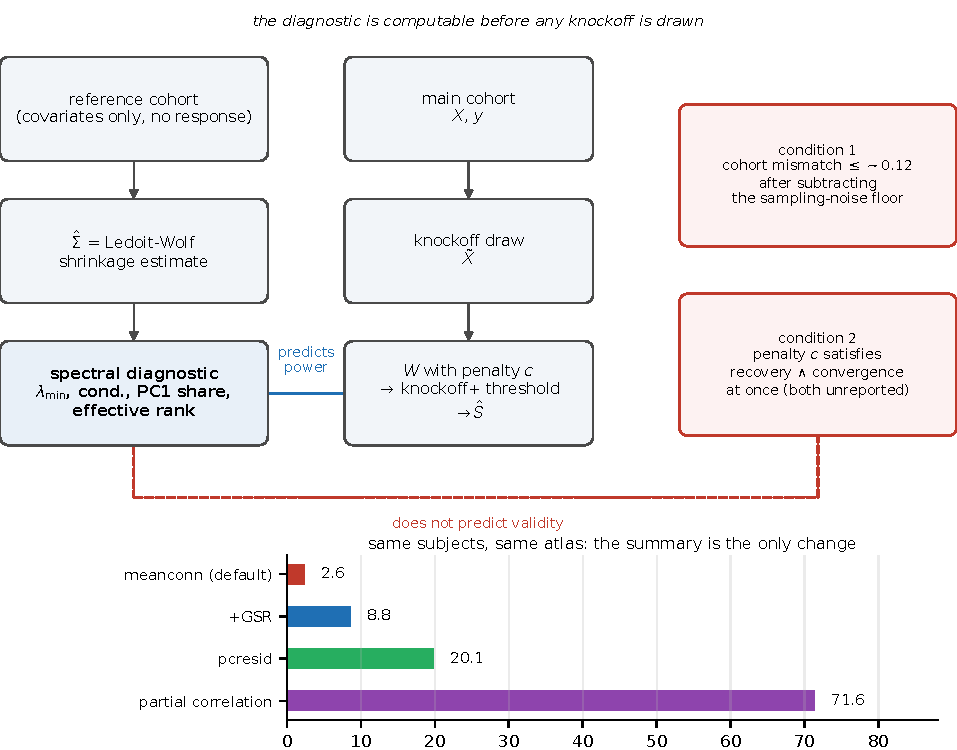
\includegraphics[width=\textwidth]{figs/fig_flow.pdf}
\caption{The diagnostic is computable before any knockoff is drawn, and it
answers a narrower question than a user may expect. Left column: the reference
cohort, which carries covariates only, yields $\hat\Sigma$ and the four
spectral quantities of \S\ref{sec:diag}. Centre column: the main cohort and
the knockoff draw. Right column: the two conditions that govern
\emph{validity}, neither of which the diagnostic predicts. The diagnostic
predicts power (solid arrow); it does not predict validity (dashed arrow),
which depends on cohort mismatch and on the penalty constant satisfying two
conditions at once. Bottom: the same subjects and the same atlas under four
summary definitions, which is the quantity the rest of the paper turns on.}
\label{fig:flow}
\end{figure}

\subsection{Controls: why injection and global nulls carry the argument}
\label{sec:controls}

On real data there is no ground truth for which ROIs are genuinely
associated with a diagnosis. We therefore cannot compute a false discovery
proportion on the real response; the only error number available there is
the procedure's own report, $(1+F_\tau)/R_\tau$, which is exactly what is
under examination. Every quantitative claim about error in this paper comes
from one of two constructions in which the truth is known by construction:

\begin{itemize}[leftmargin=1.5em,itemsep=2pt]
  \item \textbf{Injection.} A response $y=\X\beta+\varepsilon$ is generated
  with $\beta$ supported on $k$ known coordinates. The remaining $p-k$ are
  null by construction, so FDP is exact.
  \item \textbf{Global null.} The response is drawn independently of $\X$, so
  every variable is null and every discovery is false by construction. Then
  $\E[\FDP]=P(\hat S\ne\emptyset)$, and knockoff$+$ guarantees this is
  $\le q$; comparing the observed rate against $q$ is a test of validity
  that requires no biological ground truth.
\end{itemize}

\noindent
Injection amplitudes are calibrated on the \emph{conditional} $|t|$ of the
injected coordinates, which is the quantity knockoffs test. This matters:
for the ROIs with the highest variance-inflation factors, a target
conditional $|t|=6$ corresponds to a marginal $|t|=48.9$, an inflation of
$8.2\times$, rising to $13.0\times$ for random supports at low signal.
Calibrating on the marginal $|t|$ injects a contrast that is almost entirely
contained in the span of the remaining columns and measures nothing about
the procedure.

All experiments use $q=0.20$, $c=0.05$ and $\ge60$ replications (typically
200). Result tables, provenance records and a script that maps each numeric
claim in this manuscript to a specific cell of a specific result file are
archived as described in the Declarations.

\section{Results}
\label{sec:results}

\subsection{The ROI summary determines the geometry of the feature space}
\label{sec:geometry}

Table \ref{tab:geometry} reports the spectrum of the reference cohort's
correlation matrix for four summary definitions across five
dataset/parcellation combinations, and Figure \ref{fig:geometry} displays
the same quantities.

\begin{table}[htbp]
\centering
{\small\setlength{\tabcolsep}{5pt}
\begin{tabular}{lccccc}
\toprule
& & \multicolumn{4}{c}{effective rank of the reference covariance} \\
\cmidrule(lr){3-6}
dataset & $p$ & meanconn & $+$GSR & pcresid & partial \\
\midrule
ABIDE~I, AAL116, CPAC    & 113 & $2.56$ & $8.79$  & $20.06$ & $\mathbf{71.63}$ \\
ABIDE~I, AAL116, NIAK    & 116 & $3.23$ & $3.31$  & $17.97$ & $\mathbf{72.66}$ \\
ABIDE~I, CC200, CPAC     & 200 & $2.38$ & $14.71$ & $27.50$ & $\mathbf{105.16}$ \\
ABIDE~I, Harvard--Oxford & 109 & $2.23$ & $12.01$ & $22.12$ & $\mathbf{72.88}$ \\
ABIDE~II, Power2011      & 94  & $15.95$& $9.67$  & $26.36$ & $23.92$ \\
\bottomrule
\end{tabular}}
\caption{Effective rank $(\sum\lambda_i)^2/\sum\lambda_i^2$ of the reference
cohort's correlation matrix, by ROI summary definition. The conventional
definition sits at the bottom of the range in every ABIDE~I configuration.}
\label{tab:geometry}
\end{table}

\begin{figure}[htbp]
\centering
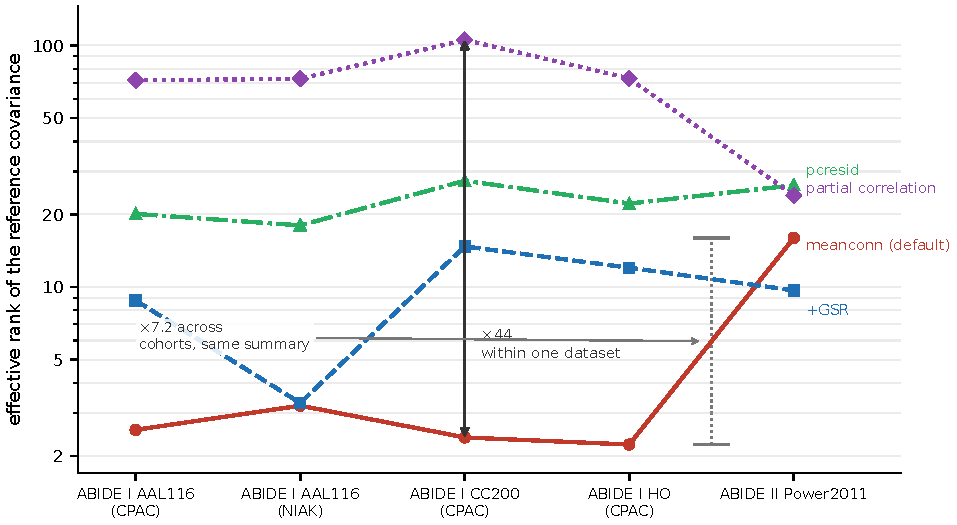
\includegraphics[width=\textwidth]{figs/fig_geometry.pdf}
\caption{The ROI summary, not the cohort, sets the geometry of the feature
space. Effective rank $(\sum\lambda_i)^2/\sum\lambda_i^2$ of the reference
cohort's correlation matrix, one line per ROI summary definition, across five
dataset/parcellation combinations (logarithmic axis; exact values in
Table~\ref{tab:geometry}). Changing the summary moves the effective rank by up
to a factor of $44$ within a single dataset; changing the dataset or
parcellation while holding the summary fixed moves it by at most a factor of
$7.2$. The convention is the binding choice.}
\label{fig:geometry}
\end{figure}

The mechanism is elementary and worth stating, because it is what makes the
result a property of the definition rather than of functional connectomes.
Feature \eqref{eq:meanconn} is a row mean of a correlation matrix. In a
correlation matrix whose leading eigenvalue is large, the row mean of row
$j$ is dominated by the $j$-th entry of the leading eigenvector, and the
vector of row means is therefore a proxy for that eigenvector. In our data
the first component carries $62\%$ of the total variance, the effective rank
is $2.56$ of $113$, and the median $R^2$ of a single feature on PC1 alone is
$0.677$, against $0.288$, $0.067$ and $0.018$ for GSR, pcresid and partial
correlation respectively (Figure~\ref{fig:mechanism}).

That the row sum of a connectivity matrix is dominated by its first
principal component is not new as a general observation: it has been
established at the group level for normative connectivity matrices
\citep{vandenheuvel2025lnm}, where the first three components exceed $70\%$
of the variance and degree correlates with PC1 at $|r|=0.82$, and for
mean-connectivity maps, where the correlation is $r=0.86$ without
global-signal regression \citep{moujaes2024ketamine}. What we add is the
per-subject, per-feature quantification---effective rank as a single
number, and the distribution of $R^2$ over features---and the consequence
in a variable-selection setting.

\begin{figure}[htbp]
\centering
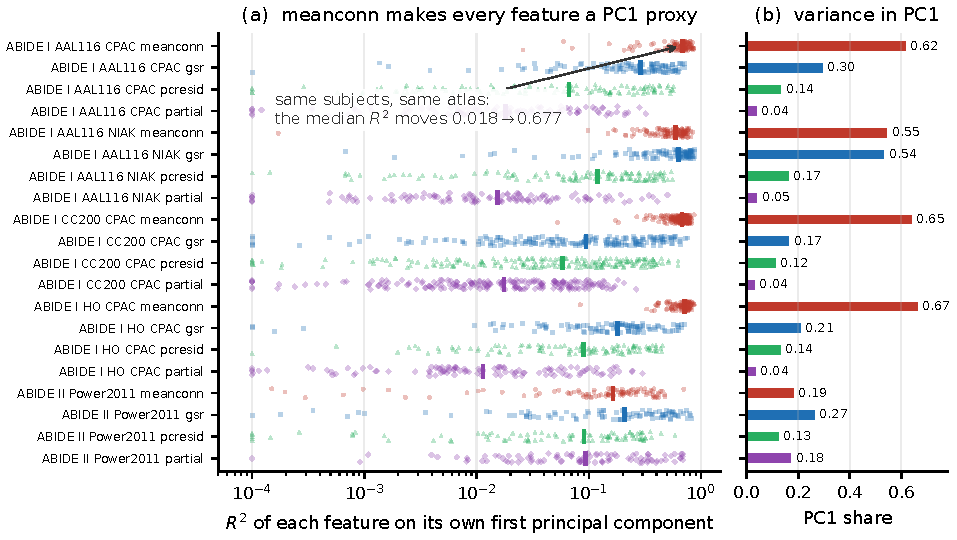
\includegraphics[width=\textwidth]{figs/fig_mechanism.pdf}
\caption{The conventional summary makes every feature a proxy for the leading
principal component; partial correlation does not. (a) One row per
dataset/summary configuration (logarithmic axis); each point is one ROI's
$R^2$ on its own principal component, computed on the reference cohort, and
the vertical bar marks the median. Holding subjects and atlas fixed (ABIDE~I,
AAL116, CPAC) the median moves from $0.018$ for partial correlation to $0.677$
for meanconn. ABIDE~II is shown as it is: its conventional summary sits at a
median of $0.164$, which is the cohort-dependence that \S\ref{sec:third}
takes up. (b) The same configurations by PC1 share.}
\label{fig:mechanism}
\end{figure}

\paragraph{The choice is not a refinement.}
The four summaries are almost mutually uncorrelated at the ROI level
(Table \ref{tab:agree}): median per-ROI Pearson correlation between $0.00$
and $0.26$, with \emph{every one} of $113$ ROIs below $0.5$. For comparison,
the two preprocessing pipelines compared in \S\ref{sec:pipeline}---a
coarser manipulation, applied to the same subjects in the same
atlas---agree at median $r=0.436$. A reader choosing a summary is choosing
which measurement to analyse, and that choice displaces the features further
than any subsequent statistical decision we examine in this paper. The
constructive version of this observation is known in the prediction
literature: no single functional-connectivity measure consistently
outperforms the others, and concatenating several is more consistent than
any one \citep{mohanty2020rethinking}.

\begin{table}[htbp]
\centering
{\small\setlength{\tabcolsep}{6pt}
\begin{tabular}{lccc}
\toprule
pair of summaries (ABIDE~I, AAL116, CPAC) & median per-ROI $r$ & min & ROIs with $r<0.5$ \\
\midrule
meanconn vs.\ GSR       & $0.219$ & $-0.109$ & $113/113$ \\
meanconn vs.\ pcresid   & $-0.129$& $-0.317$ & $113/113$ \\
meanconn vs.\ partial   & $0.210$ & $0.014$  & $113/113$ \\
GSR vs.\ partial        & $0.005$ & $-0.205$ & $113/113$ \\
partial vs.\ pcresid    & $0.114$ & $-0.026$ & $113/113$ \\
\bottomrule
\end{tabular}}
\caption{Agreement between ROI summary definitions, per ROI, over the same
subjects. The summaries are effectively different measurements.}
\label{tab:agree}
\end{table}

\paragraph{The conventional neuroimaging remedy is not reliable.}
Global-signal regression, the field's standard response to the global
component, raises the effective rank on ABIDE~I CPAC ($2.56\to8.79$), does
nothing on the NIAK pipeline ($3.23\to3.31$), and \emph{lowers} it on
ABIDE~II ($15.95\to9.67$). The contrast with the ABIDE~I direction is
robust: over five random reference-cohort splits the ABIDE~I effect is
$2.49\pm0.08\to9.08\pm0.47$ and the ABIDE~II effect is
$17.20\pm1.18\to11.18\pm0.52$. It is not a rank-ceiling artefact---ABIDE~II
has $T\ge119$ for every subject against $p=94$, so no subject is in the
$T\le p$ regime---and we do not have a mechanism for it. We flag it because
it runs opposite to the published expectation that removing the global
signal removes the dominant mode \citep{moujaes2024ketamine}, and because
the direction of a GSR effect on connectivity structure is contested on
other grounds: GSR is known to create group differences that favour one
group, remove the strongest true differences, and displace the location of
group effects \citep{gotts2013perils,saad2012trouble,ciric2017benchmarking},
while its motion-attenuation benefit is real
\citep{ciric2017benchmarking,murphy2017consensus}. The defensible reading is
that GSR is a choice with consequences in both directions rather than a
correction. Removing the leading principal components worked in every
configuration we tried.

\subsection{The received explanation fails its own test}
\label{sec:boundary}

If the spectral collapse caused the null results, a simulation using the
collapsed covariance should return nothing. It does not.
Table~\ref{tab:boundary} sweeps the covariance from the ABIDE structure to
the identity, and across AR(1) structures and the twenty real feature
matrices of Table~\ref{tab:geometry}, holding the pipeline fixed.
Figure~\ref{fig:limits}a,b shows the same sweep on the effective-rank axis,
where the invariance is visible at a glance.

\begin{table}[htbp]
\centering
{\small\setlength{\tabcolsep}{6pt}
\begin{tabular}{llccc}
\toprule
& & effective rank & power & FDP \\
\midrule
\multirow{3}{*}{A: $\Sigma(t)=(1-t)\Sigma_{\mathrm{ABIDE}}+tI$}
 & $t=0$   & $2.56$  & $\mathbf{0.859}$ & $0.154$ \\
 & $t=0.10$& $3.15$  & $0.974$ & $0.132$ \\
 & $t=1$   & $113.0$ & $1.000$ & $0.176$ \\
\midrule
B: AR(1), $\rho\in[0.02,0.80]$ & --- & $25$--$113$ & $1.000$ & $0.17$--$0.20$ \\
\midrule
C: 20 real feature matrices & --- & $2.23$--$105$ & $0.770$--$1.000$ & $0.15$--$0.21$ \\
\bottomrule
\end{tabular}}
\caption{Power and realised FDP against covariance conditioning, pipeline
held fixed ($n_{\mathrm{ref}}=393$, $n_{\mathrm{main}}=459$, $q=0.20$,
$c=0.05$, $k=12$, $200$ replications; every configuration fully converged).
Using the real ABIDE covariance as ground truth gives power $0.859$, not
zero. Across all $41$ configurations the minimum power is $0.770$, attained
by the NIAK $+$ GSR combination that Table~\ref{tab:geometry} identifies as
the one case where GSR fails to help.}
\label{tab:boundary}
\end{table}

\noindent
The spectral collapse is real and it costs something---$0.859$ against
$1.000$, about fourteen percentage points---but it does not make the
procedure powerless. Whatever produced the null results on real data, it was
not the conditioning of the covariance. This matters because the two
readings are easy to hold at once and they contradict each other: the same
covariance can be described as degenerate enough that no construction should
work, and yet deliver per-signal power of $0.859$; those two statements
cannot both hold, and this experiment is the resolution.

\subsection{What limits power is the number of true signals}
\label{sec:limits}

The same conclusion holds when signals are injected into the \emph{real}
covariates. Table~\ref{tab:control} reports per-signal power by covariance
arm and support size; Figure~\ref{fig:limits}c shows the same contrast
against the strength of the injected signal, which is the factor that does
move power.

\begin{table}[htbp]
\centering
{\small\setlength{\tabcolsep}{5pt}
\begin{tabular}{lcccc}
\toprule
support & conditional $|t|$ & ref ($n=100$) & ref ($n=393$)
 & main as its own ref \\
\midrule
\multirow{3}{*}{random, $k=12$}
 & $3$ & $0.59$ & $0.68$ & $0.69$ \\
 & $4$ & $0.79$ & $0.88$ & $0.89$ \\
 & $6$ & $0.93$ & $\mathbf{0.98}$ & $\mathbf{0.98}$ \\
\midrule
random, $k=3$            & $6$ & $0.16$ & $0.21$ & $0.19$ \\
near-collinear, $k=3$    & $6$ & $0.13$ & $0.28$ & $0.24$ \\
\bottomrule
\end{tabular}}
\caption{Per-signal power (fraction of injected coordinates recovered) on
real ABIDE~I covariates, by covariance arm. Enlarging the reference cohort
has a small monotone effect that is visible at moderate signal---at
conditional $|t|=3$, $k=12$, per-signal power rises from $0.590$ at
$n_{\mathrm{ref}}=100$ to $0.676$ with the full reference cohort---and
narrows as the signal strengthens, which is the direction the theory predicts
since a noisier $\hat\Sigma$ is the more conservative one
\citep{candes2018panning}. So \textbf{the reference cohort is a secondary
constraint, not the binding one}. At fixed covariance and signal strength,
the dominant factor is $k$. The last column is a \emph{reference point, not a
recommended procedure}: it estimates $\hat\Sigma$ from the same covariates
that enter the statistic, so it does not meet the known-$F_X$ requirement and
its FDR control is not guaranteed by the theory. Its realised FDP
($0.04$--$0.15$, inside $q=0.20$) is nonetheless unsurprising, because
\citet{barber2020robust} bound the inflation by the divergence between the
true and working conditional distributions, and that divergence here has one
source---finite-sample estimation---rather than the two the reference-cohort
arms carry. We use it to ask what reference data buys in power, and nothing
else. The
near-collinear support---the three ROIs with the highest variance-inflation
factors in the atlas---does no worse than a random support of the same size,
so the degeneracy of the features does not limit power in the specific
directions we can measure.}
\label{tab:control}
\end{table}

\noindent
Two facts emerge. Reference-cohort size has only a small effect, and only
where the signal is weak enough for $\hat\Sigma$'s noise to matter: at
conditional $|t|=3$, $k=12$, per-signal power is $0.590$ at
$n_{\mathrm{ref}}=100$ against $0.676$ for the full cohort, and the three arms
converge to $0.93$/$0.98$/$0.98$ by $|t|=6$. The factor that does move power
is the number of true signals, from $0.97$ at $k=12$ to $0.20$ at $k=3$ under
identical signal strength. This is knockoff$+$'s own conservatism: the
threshold in \eqref{eq:tau} requires $R\ge(1+F)/q$, which is hard to satisfy
when few coordinates are non-null. It is a property of the method, not of
the covariance and not of the reference cohort. The dependence is
qualitatively consistent with the first-passage characterisation of the
knockoff$+$ threshold \citep{zhang2026mirror}; we note that the asymptotic
power theory in \citet{weinstein2023power} assumes the number of non-nulls
grows with $p$, a regime our $k=3$ configurations are outside.

\begin{figure}[htbp]
\centering
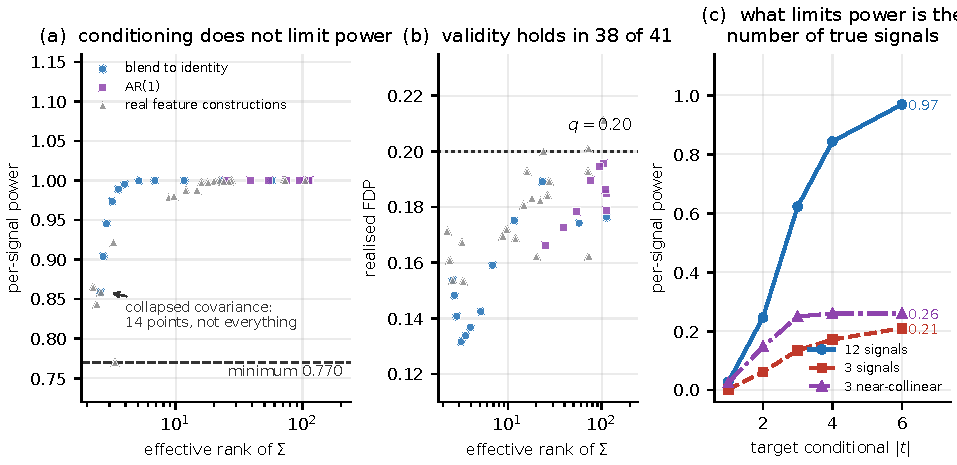
\includegraphics[width=\textwidth]{figs/fig_limits.pdf}
\caption{Conditioning does not limit power; the number of true signals does.
(a) Per-signal power against the effective rank of $\Sigma$ over all $41$
covariance configurations of Table~\ref{tab:boundary} and three construction
families, spanning effective rank $2.2$ to $113$; the dashed line is the
minimum over the whole set. The most collapsed covariance costs $14$ points of
power---it does not return nothing. (b) The realised FDP over the same
configurations; the guarantee holds in $38$ of $41$, so validity is not the
constraint here either. (c) The factor that does move power: per-signal power
against the target conditional $|t|$ of the injected signal, for $12$ random
signals, $3$ random signals, and $3$ near-collinear signals. The number of
true signals, not the conditioning, sets the ceiling. Panels are on different
x-scales; (a) and (b) share one.}
\label{fig:limits}
\end{figure}

\subsection{Exhausting the alternatives}
\label{sec:exhaust}

If the limitation is not the reference cohort, it is worth establishing that
it is not any of the other obvious candidates either. We tested three
classes of alternative. The first two---knockoff constructions and Gaussian
mirrors---share one positive control and are compared in
Figure~\ref{fig:machinery} on the two axes that matter at once, power and
validity; the third is treated separately below because it reports selections
rather than an error rate.

\paragraph{Knockoff constructions.} Table~\ref{tab:construct} reports the
construction diagonal $s$ for six methods on degenerate and non-degenerate
features. On the degenerate features the six constructions are
indistinguishable: median $s$ between $0.063$ and $0.088$, implying
$\mathrm{Corr}(X_j,\Xt_j)$ between $0.912$ and $0.937$. Every construction
is forced into the same near-replica regime, and the SDP solution is not
better---it minimises $s$ on some coordinates, returning $s=0$ for the
coordinates it sacrifices. This is the rank deficiency that
\citet{spector2022powerful} identify, appearing here as a ceiling on what
any construction can achieve when $\Sigma$ is nearly singular. On the
less-degenerate features the construction matters a great deal: on ABIDE~II
partial-correlation features, SDP raises $s$ to $4.6$ times the
equicorrelated value.

\begin{table}[htbp]
\centering
{\small\setlength{\tabcolsep}{5pt}
\begin{tabular}{lcccccc}
\toprule
& \multicolumn{6}{c}{median $s$ (and $\mathrm{Corr}(X_j,\Xt_j)=1-s$)} \\
\cmidrule(lr){2-7}
configuration & equi & identity & SDP & ASDP & MVR & ME \\
\midrule
AAL116 meanconn ($\ld=0.032$) & $0.064$ & $0.064$ & $0.088$ & $0.063$ & $0.069$ & $0.081$ \\
ABIDE~II partial ($\ld=0.067$) & $0.133$ & $0.133$ & $\mathbf{0.611}$ & $0.294$ & $0.431$ & $0.511$ \\
\bottomrule
\end{tabular}}
\caption{Knockoff constructions compared at matched data. On degenerate
features all six are indistinguishable, and SDP returns $s=0$ on the
coordinates it sacrifices. On less-degenerate features the choice matters
by a factor of $4.6$.}
\label{tab:construct}
\end{table}

\paragraph{A method that never inverts $\Sigma$.} Gaussian mirrors
\citep{xing2023gaussian} construct, for each variable, a pair of mirror
variables $x_j^\pm = x_j \pm c_j z_j$ with $z_j\sim N(0,I_n)$ and $c_j$
chosen so that the mirror statistic is exactly symmetric under the null. The
construction never forms $\Sigma^{-1}$, so the spectral collapse cannot
enter it. On our features it is \emph{valid}---under a global null it
returns a nonempty selection in $8.0\%$ of replications, within
$q=0.20$---but it recovers only $0.421$ of injected signals against
$0.977$ for the knockoff filter, at FDP $0.000$ against $0.110$. The reason
is measurable and is the same geometry: $c_j$ is set by the residual of
$x_j$ on all other columns, whose norm is $6.60$ against $\|x_j\|=21.4$,
so each variable is $90.5\%$ explained by the others. A method designed to
avoid $\Sigma^{-1}$ fails at the same place, which is direct evidence that
the inversion is not the binding constraint.

\paragraph{Cross-environment consistency.} The multi-environment knockoff
filter \citep{li2022multienv} tests not ``is this ROI associated with
diagnosis'' but ``in how many environments is it consistently associated'',
with FDR control. This matches our setting, where the strongest observation
is that nothing is consistent. Using the eight ABIDE~I sites with $n\ge40$
and both diagnostic classes as environments, and estimating $\Sigma$ from
the remaining environments in each case, no ROI is selected at any
consistency level $r\in\{1,\dots,5\}$, and a negative control that permutes
the response within each environment also returns nothing.

That zero is uninformative, and we established why before reading it as a
result. Unlike every other alternative in this section, this arm has a
positive control: we injected a signal that is consistent across environments
by construction---the same twelve coordinates, the same sign and the same
standardised effect size in every site, calibrated to a conditional $|t|$ of
$6$ as elsewhere in this paper---and ran the filter on it over $60$
replicates. In the configuration above the filter recovers a mean of $0.100$
of the injected coordinates at best ($r=2$, $c=0.05$) and nothing at all at
$c=0.15$, while the permuted control returns nothing in either case. The
limitation is the size of the environments rather than the filter: pooling
the same subjects into four groups of about $213$ rather than eight sites of
$42$--$169$, the identical injected signal is recovered at a mean rate of
$0.762$ at $r=1$ and $0.736$ at $r=2$. With $p=113$ and every site holding
fewer than $170$ subjects, the per-environment knockoff fits are too weak to
yield a signed statistic. We therefore read the empty selection on the real
response as showing only that this arm cannot distinguish ``no replicable
association'' from ``no power''; no other arm in this paper has that
property, and the two failures of \S\ref{sec:shift} and \S\ref{sec:penalty}
are established from controls that do have power.

\begin{figure}[htbp]
\centering
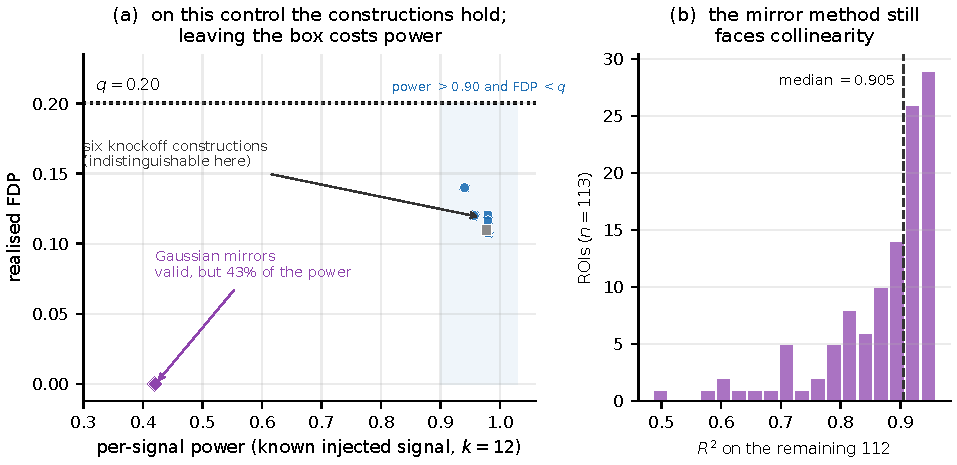
\includegraphics[width=\textwidth]{figs/fig_machinery.pdf}
\caption{Alternative constructions do not escape the trade-off. (a)
Per-signal power against realised FDP for the six knockoff constructions and
the Gaussian mirrors, all evaluated on one positive control (an injected
signal of known conditional strength, $k=12$, calibrated on the same quantity
for every arm); the shaded box is the region with power above $0.90$ and FDP
below $q$. The six constructions are indistinguishable inside it. Gaussian
mirrors leave it: they are valid---they never invert $\Sigma$---but recover
$43\%$ of the power. The matrix-power family is not on this panel because it
uses a different injection convention (\S\ref{sec:matrixpower}); there the
constructions do leave the box, and what they lose is validity rather than
power. (b) The mechanism behind the mirrors' shortfall: $R^2$ of each ROI on
the remaining $112$, median $0.905$, so avoiding $\Sigma^{-1}$ does not avoid
collinearity.}
\label{fig:machinery}
\end{figure}

\subsection{The matrix-power family: reported error and true error move in
opposite directions}
\label{sec:matrixpower}

The three alternatives above are discrete. A continuous family makes the
same point more sharply. If $\Sigma$ is a correlation matrix, the linear
transform
\begin{equation}
  \X_t \;=\; \X\,\Sigma^{(t-1)/2}
  \qquad\Longrightarrow\qquad
  \mathrm{corr}(\X_t)=\Sigma^{t},
  \label{eq:matpow}
\end{equation}
since $\Sigma^{(t-1)/2}\,\Sigma\,\Sigma^{(t-1)/2}=\Sigma^{t}$. Applied
identically to the reference and main cohorts, this is a legitimate
one-parameter family of feature representations, interpolating between the
marginal correlation ($t=1$), the whitened features ($t=0$), and the
precision ($t=-1$). The effective rank moves monotonically across it, from
$2.56$ to $111$ and back to $76$.

This family is a natural way to try to increase the discriminability of
degenerate features, and it is worth reporting what happens when one does.
Figure~\ref{fig:matrixpower} and Table~\ref{tab:matpow} give the result
under three responses: an injected
signal fixed in the \emph{original} ROI space, the real diagnosis, and a
global null.

\begin{table}[htbp]
\centering
{\small\setlength{\tabcolsep}{5pt}
\begin{tabular}{lcccccc}
\toprule
& \multicolumn{2}{c}{injection, $k=12$}
& \multicolumn{2}{c}{real response}
& \multicolumn{2}{c}{global null} \\
\cmidrule(lr){2-3}\cmidrule(lr){4-5}\cmidrule(lr){6-7}
$t$ & eff.\ rank & power / FDP & $P(\hat S\ne\emptyset)$ & reported & $P(\hat S\ne\emptyset)$ & true FDP \\
\midrule
$1.0$  & $2.56$  & $0.892$ / $0.130$ & $0.355$ & $0.250$ & $0.055$ & $1.00$ \\
$0.6$  & $17.63$ & $0.957$ / $0.493$ & $0.540$ & $0.200$ & $0.045$ & $1.00$ \\
$0.2$  & $97.93$ & $0.965$ / $0.808$ & $0.790$ & $0.143$ & $0.075$ & $1.00$ \\
$0.0$  & $111.09$& $0.954$ / $0.826$ & $0.875$ & $0.125$ & $0.100$ & $1.00$ \\
$-0.6$ & $94.70$ & $0.881$ / $0.766$ & $0.980$ & $0.091$ & $\mathbf{0.280}$ & $1.00$ \\
$-1.0$ & $76.10$ & $0.790$ / $0.726$ & $0.985$ & $0.100$ & $0.245$ & $1.00$ \\
\bottomrule
\end{tabular}}
{\small \emph{``reported''} is the median of the procedure's own threshold
ratio $\min_t(1+F_t)/R_t$; under a global null the true FDP is $1$ whenever
anything is reported, so $P(\hat S\ne\emptyset)$ \emph{is} the expected FDP
and must be compared against $q=0.20$.}
\caption{The matrix-power family \eqref{eq:matpow}. Power on a fixed
injected signal is flat across the whole range ($0.79$--$0.97$); what moves
is the false discovery count. The two monotone columns tell the story: the
procedure's own reported error improves from $0.250$ to $0.091$ while the
true error rises from $0.130$ to $0.826$, and under a global null the rate
of nonempty selections crosses the nominal level between $t=-0.2$ and
$t=-0.4$.}
\label{tab:matpow}
\end{table}

\begin{figure}[htbp]
\centering
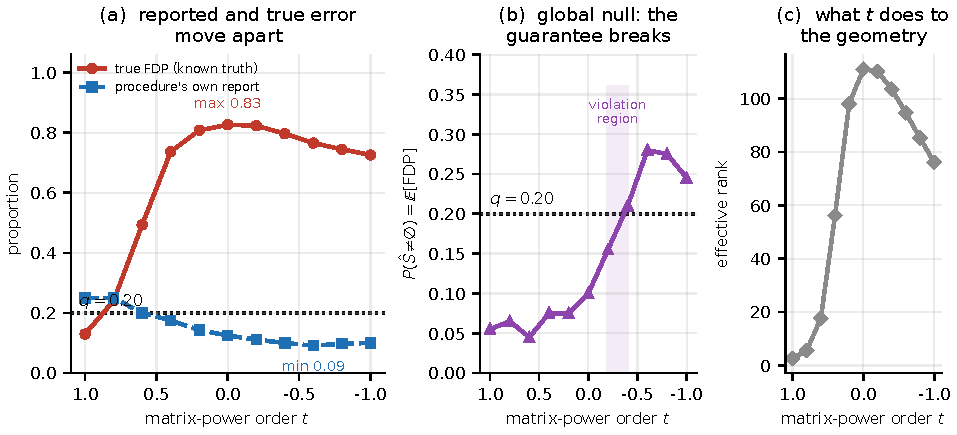
\includegraphics[width=\textwidth]{figs/fig_matrixpower.pdf}
\caption{Along the matrix-power family the procedure's own report and its
true error move in opposite directions. (a) Under an injected signal whose
truth is known, the realised FDP (red, solid) rises to $0.826$ while the
procedure's own reported threshold ratio (blue, dashed) falls to $0.091$;
both are proportions, so they share an axis. (b) Under a global null the true
FDP is $1$ whenever anything is reported, so the curve \emph{is} the expected
FDP; it crosses $q=0.20$ between $t=-0.2$ and $t=-0.4$ (shaded). (c) What $t$
does to the geometry, so that the family can be read on the effective-rank
scale of \S\ref{sec:geometry}. Series are distinguished by marker and line
style as well as colour, so the figure survives grayscale printing.}
\label{fig:matrixpower}
\end{figure}

Three readings, in increasing order of importance. The transform does not
help: power is flat, so it does not make true signal easier to find. It
hurts in a way that is invisible: at $t=0$ the procedure reports a threshold
ratio of $0.125$, comfortably inside $q$, while committing a false discovery
proportion of $0.826$. And the global-null column closes the argument
without appealing to any biological ground truth: with a response drawn
independently of the covariates, the rate of nonempty selections rises from
$0.055$ at $t=1$ to $0.280$ at $t=-0.6$, crossing $q=0.20$; since every
discovery in that column is false by construction, this is a direct
violation of the guarantee. A user tuning $t$ by the two quantities the
software shows them---number of discoveries and reported ratio---would be
led to $t\approx-0.6$, where the true error is $0.77$.

\subsection{Cohort shift breaks validity without reducing power}
\label{sec:shift}

The simulations above draw both cohorts from one $\Sigma$, which measures
estimation error only. The subject of this paper is a reference cohort that
is \emph{different}. We draw $\X_{\mathrm{ref}}\sim N(0,\Sigma)$ and
$\X_{\mathrm{main}}\sim N(0,\Sigma_\delta)$ with $\Sigma_\delta=
\mathrm{pd}\big((1-\delta)\Sigma+\delta P\big)$ for a sparse random
perturbation $P$.

\begin{table}[htbp]
\centering
{\small\setlength{\tabcolsep}{6pt}
\begin{tabular}{lcccc}
\toprule
$\delta$ & mismatch & power & realised FDP \\
\midrule
$0.00$ & $0.000$ & $0.859$ & $0.154$ \\
$0.10$ & $0.062$ & $0.966$ & $0.144$ \\
$0.20$ & $0.124$ & $0.994$ & $0.180$ \\
$0.30$ & $0.186$ & $1.000$ & $\mathbf{0.227}$ \\
$0.80$ & $0.497$ & $0.999$ & $\mathbf{0.422}$ \\
\bottomrule
\end{tabular}}
\caption{Cohort distribution shift. Mismatch is the RMS difference of the
off-diagonal correlation entries. The observed ABIDE~I mismatch between the
main and reference cohorts is $0.0593$, corresponding to $\delta\approx0.10$
(row 2), where FDP is $0.144$.}
\label{tab:shift}
\end{table}

\begin{figure}[htbp]
\centering
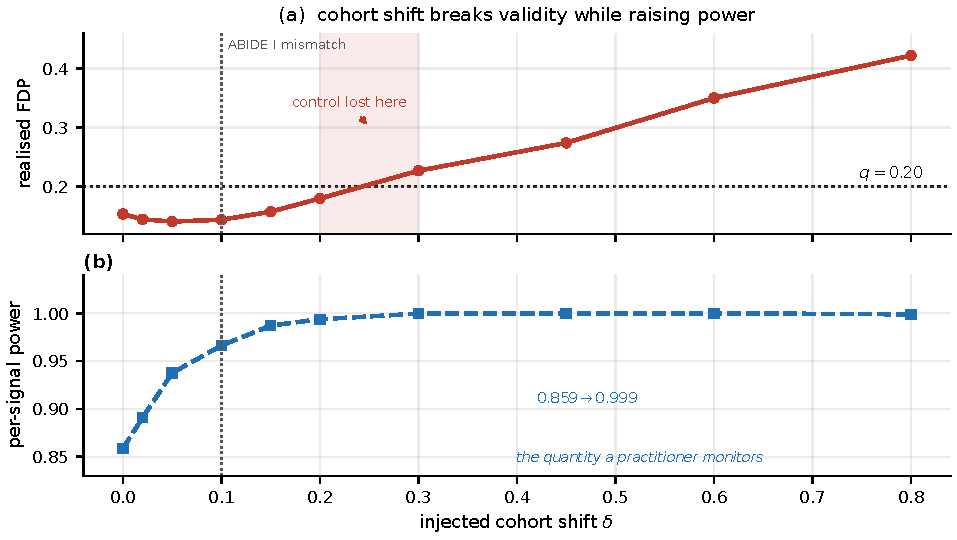
\includegraphics[width=\textwidth]{figs/fig_shift.pdf}
\caption{Cohort shift breaks validity while raising power. (a) Realised FDP
against the injected cohort shift $\delta$; the shaded band marks the interval
between the last level at which FDP is controlled and the first at which it is
not, and the dotted line marks the grid level whose simulated mismatch,
$0.062$, is closest to the $0.059$ observed in ABIDE~I. (b)
Per-signal power over the same shift, which rises throughout. A user
monitoring the quantity in (b) reads this failure as improvement; the failure
is silent because the quantity they watch moves the wrong way.}
\label{fig:shift}
\end{figure}

\noindent
The failure mode is specific (Figure~\ref{fig:shift}). As the cohorts
diverge, power \emph{rises}
from $0.859$ to $0.999$ while the realised FDP rises from $0.154$ to
$0.422$. Apparent power grows because knockoffs built from a mismatched
covariance are less correlated with the originals, so the statistic
separates them more easily; the same mechanism destroys the calibration. A
user watching only the discovery count reads this as improvement. FDP
control is lost between $\delta=0.20$ and $\delta=0.30$ (mismatch
$0.124$--$0.186$; we did not resolve the crossing more finely than the
grid), and the observed ABIDE~I mismatch of $0.0593$ sits inside the safe
region---which is why this failure mode does not explain our null results
either. It would have produced \emph{more} discoveries, not fewer.

The precise condition this violates is worth naming. Knockoff validity
requires exchangeability under the conditional law $L(\X\mid Y)$, whereas a
reference cohort supplies a distribution valid under the marginal $P(\X)$;
when the sampling law differs from the population law the implication
breaks \citep{zhao2025tilted}. This is the imaging analogue of the
reference-panel mismatch that GWAS knockoff methods must contend with
\citep{chen2021ldref,kanai2022slalom,benner2017finemap}.

\subsection{The penalty constant must satisfy two conditions}
\label{sec:penalty}

The fixed-$\lambda$ statistic \eqref{eq:lcd} has one tuning parameter, and
we chose it badly at the outset of this analysis. Holding data,
knockoffs, covariance and solver fixed and varying only $c$
(Figure~\ref{fig:penalty}):

\begin{table}[htbp]
\centering
{\small\setlength{\tabcolsep}{6pt}
\begin{tabular}{lccc}
\toprule
& \multicolumn{2}{c}{constraint 1: the signal must survive}
& constraint 2: the solver must converge \\
\cmidrule(lr){2-3}\cmidrule(lr){4-4}
$c$ & recovered (of $12$) & all $12$ recovered & non-convergence, real response \\
\midrule
$0.02$ & $11.97$ & $0.97$ & $96.7\%$--$100\%$ \\
$0.03$ & $11.97$ & $0.97$ & $\mathbf{13.3\%}$--$\mathbf{46.7\%}$ \\
$0.05$ & $11.73$ & $0.80$ & $\mathbf{0\%}$ \\
$0.10$ & $6.95$  & $0.13$ & $0\%$ \\
$0.15$ & $\mathbf{1.12}$ & $0.02$ & $0\%$ \\
$0.30$ & $0.07$  & $0.00$ & $0\%$ \\
\bottomrule
\end{tabular}}
\caption{The penalty constant must satisfy two constraints at once, and
they pull in opposite directions. Constraint 1 is measured by injecting
signals of known conditional strength ($k=12$, conditional $|t|=6$, $60$
replications) and counting how many coordinates are recovered; constraint 2
is measured on the real (weak) response, where a small penalty yields a
dense lasso and coordinate descent may exhaust its iteration budget. Neither
constraint is reported by the software. Only $c=0.05$ satisfies both.}
\label{tab:penalty}
\end{table}

\begin{figure}[htbp]
\centering
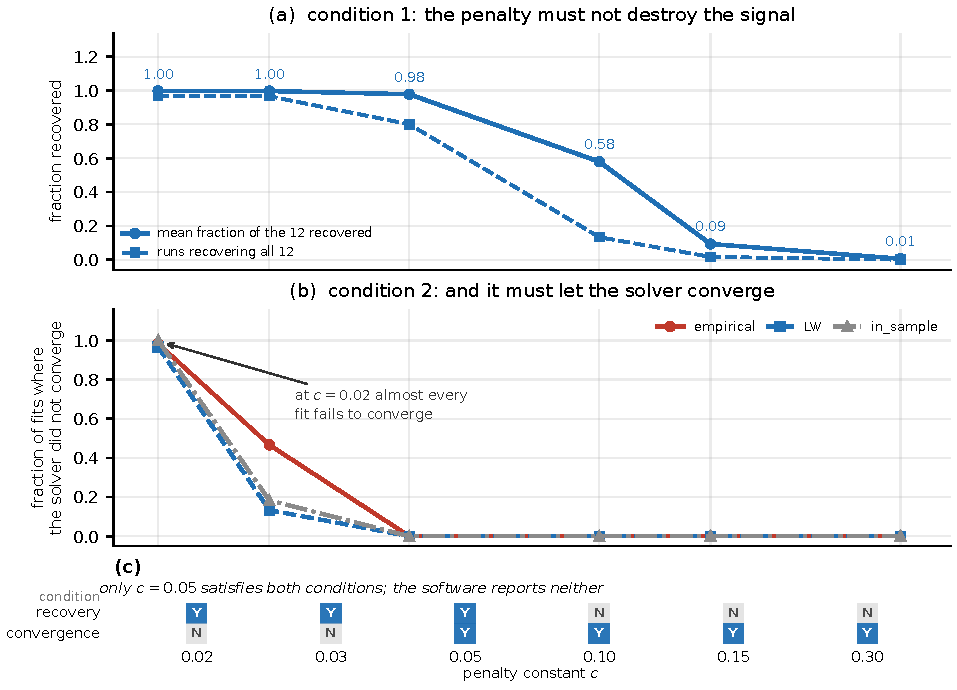
\includegraphics[width=\textwidth]{figs/fig_penalty.pdf}
\caption{The penalty constant must satisfy two conditions at once, and they
pull in opposite directions. (a) Fraction of the $12$ injected signals
recovered, against $c$ (logarithmic axis), shown both as the mean fraction
recovered (solid) and as the fraction of runs in which all twelve are
recovered (dashed); both collapse beyond $c=0.05$. (b) Fraction of fits in
which the solver failed to converge on the real response, for the empirical
covariance and for two Ledoit--Wolf variants (\S\ref{sec:diag}); below
$c=0.05$ almost every fit fails. (c) The conjunction, taking recovery as a
mean fraction of at least $0.90$: only $c=0.05$ satisfies both conditions, and
the software reports neither, so the failure is invisible unless both are
checked deliberately.}
\label{fig:penalty}
\end{figure}

\noindent
A signal whose conditional $|t|$ reaches $6$ is almost entirely penalised
away at $c=0.15$: $1.12$ of $12$ coordinates are recovered on average, and
all twelve are recovered in only $2\%$ of replications. Reducing $c$ fixes
that, but on the real response the penalty also controls how dense the
solution is, and the real response is weak: at $c=0.02$ the solver exhausts
the iteration cap in $96.7\%$--$100\%$ of runs and at $c=0.03$ in up to
$46.7\%$, returning a statistic that has not converged and should not be
interpreted. Only $c=0.05$ both recovers the injected signal ($11.73$ of
$12$) and converges on the real response, with $2.4\times$ iteration
headroom.

We note that this is a regime our power theory does not cover. Asymptotic
analyses of the penalty-power relationship assume an i.i.d. design and often
recommend cross-validated tuning \citep{weinstein2023power}; on data with
$p/n=0.25$ and a highly correlated $\Sigma$ the relation is not monotone in
the way those results assume, and the relevant fragility has been documented
for the one-standard-error rule \citep{candes2018panning}.

\subsection{Real-data answers are distributions, not numbers}
\label{sec:draws}

Knockoff generation is random. It is tempting, and common, to report the
discovery count from a single draw; the numbers below show why that is an
artefact. A single draw returning $\hat S=\emptyset$ reads as ``yields no
discoveries'', while the same configuration measured over repeated draws
returns nothing in $64.5\%$ of them and up to $28$ regions in the rest. The
two statements cannot both stand, and the first is the one an author is more
likely to report.

Holding everything except the draw fixed ($c=0.05$, $200$ draws per
configuration), the real-response results are (Figure~\ref{fig:draws}):

\begin{table}[htbp]
\centering
{\small\setlength{\tabcolsep}{5pt}
\begin{tabular}{llccccc}
\toprule
dataset & summary & $P(\hat S\ne\emptyset)$ & median $|\hat S|$ & max $|\hat S|$
 & median ratio & converged \\
\midrule
ABIDE~II, Power2011 & \textbf{pcresid} & $\mathbf{0.815}$ & $\mathbf{12}$ & $40$ & $\mathbf{0.148}$ & $1.00$ \\
ABIDE~I, Harvard--Oxford & meanconn & $0.420$ & $0$ & $24$ & $0.250$ & $1.00$ \\
ABIDE~I, AAL116, CPAC & meanconn & $0.355$ & $0$ & $28$ & $0.250$ & $1.00$ \\
ABIDE~II, Power2011 & meanconn & $0.190$ & $0$ & $20$ & $0.369$ & $1.00$ \\
ABIDE~I, AAL116, CPAC & partial & $0.010$ & $0$ & $5$ & $0.742$ & $1.00$ \\
ABIDE~I, AAL116, NIAK & GSR & $0.000$ & $0$ & $0$ & $0.857$ & $1.00$ \\
\bottomrule
\end{tabular}}
\caption{Distribution of knockoff selections on the real ASD/control
response, $200$ independent draws per configuration with the pipeline
otherwise fixed. The reported ratio is $\min_t(1+F_t)/R_t$, the optimal
attainable threshold ratio. One of the twenty configurations we ran (CC200
with meanconn features, convergence rate $0.37$) is excluded for
non-convergence; all rows shown are fully converged. \textbf{These are not
discoveries}: on real data we have no ground truth for which ROIs are
genuinely associated with diagnosis, so the selections cannot be validated
and we make no claim about them. They are reported because the
\emph{distribution} is the honest output of the procedure, and because the
spread across configurations is itself the finding.}
\label{tab:draws}
\end{table}

\begin{figure}[htbp]
\centering
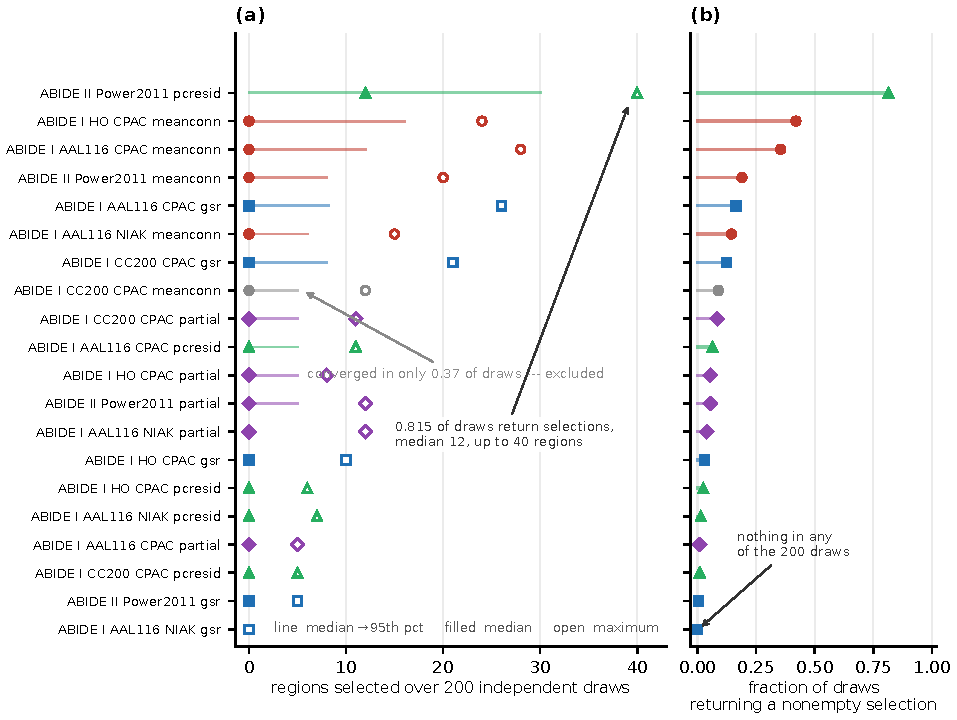
\includegraphics[width=\textwidth]{figs/fig_draws.pdf}
\caption{The output of the procedure on the real response is a distribution,
not a number. (a) One row per dataset/summary configuration, ordered by the
fraction of draws returning a nonempty selection; the thin line spans the
median to the $95$th percentile of $|\hat S|$, the filled dot marks the
median and the open dot the maximum over $200$ independent knockoff draws.
The grey row is excluded: its solver converged in only $0.37$ of draws. Of the
twenty configurations, nineteen have a median of zero; eighteen of them
nevertheless reach a nonzero maximum, and one returns nothing in any draw.
(b) The same rows, showing that fraction directly. The top row returns
selections in $0.82$ of draws and up to $40$ regions; the bottom row returns
nothing in any draw---same procedure, same response, same $q$, a different
summary. $P(\hat S\ne\emptyset)$ equals the fraction of draws whose optimal
ratio falls below $q$, so panels (a) and (b) encode one quantity, not two.
These are not discoveries: on real data no ground truth exists, so the
spread across configurations is itself the finding.}
\label{fig:draws}
\end{figure}

\noindent
Two readings. First, ``no discoveries'' is not a property of this data: the
conventional meanconn features on AAL116 return a nonempty selection in
$35.5\%$ of draws and as many as $28$ regions, and the Harvard--Oxford
parcellation is higher still. A single-draw analysis would have justified
the opposite conclusion, which is why we report the whole distribution. Second, the output depends on the feature definition far more
than on anything else we varied: from $P(\hat S\ne\emptyset)=0.000$ for NIAK
GSR to $0.815$ for ABIDE~II pcresid. The procedure's own reported ratio
ranges from $0.148$ (inside $q$) to $0.857$ (far outside), so the
\emph{feasibility} of a controlled selection at $q=0.20$ is also
feature-dependent. We emphasise again that the $0.815$ configuration is not
a discovery claim: it is a claim about what the procedure reports, from a
procedure whose report we have shown to be unreliable under other
manipulations (\S\ref{sec:matrixpower}, \S\ref{sec:shift}).

\subsection{Two properties supported by controls}
\label{sec:retained}

Two further properties follow from the same controls and are worth stating
separately, because both are easy to get wrong.

\paragraph{Aggregating draws by averaging the statistics is invalid.}
Median aggregation across $M$ independent knockoff draws removes the
zero-discovery runs entirely and more than doubles mean pairwise Jaccard
similarity, so it appears to work. Under a global null it returns a median
of $20.6$ discoveries at $M=10$ with a realised FDP of $0.97$, while the
$e$-value construction of \citet{ren2024derandomised},
\begin{equation}
  e_j = p\cdot\frac{\mathbf{1}\{W_j\ge T\}}{1+\#\{k:W_k\le -T\}},
  \label{eq:eval}
\end{equation}
with e-BH \citep{wang2022ebh} applied to the averaged $e$-values, returns
nothing---the correct answer. On a single draw, e-BH applied to
\eqref{eq:eval} reproduces the knockoff$+$ selection set identically in
$25$ of $25$ instances, an algebraic identity and therefore a unit test of
the implementation rather than evidence of validity.

The reason is worth recording, because the argument for median aggregation
is superficially convincing. For a null $j$ each draw's $W_j^{(m)}$ is
symmetric about zero with an independent fair sign, so the \emph{marginal}
distribution of the median is symmetric. Knockoff$+$ requires the null signs
to be jointly independent given the magnitudes, and the median does not
inherit that: its sign and magnitude are entangled through the pattern of
signs across draws. Marginal symmetry is necessary and not sufficient, and a
numerical check of marginal symmetry cannot detect the difference. This
failure is corroborated in the aggregation literature \citep{nguyen2020ako}.
We note a distinction that matters for interpretation: the median we
criticise is taken \emph{across independent knockoff draws}. Medians taken
\emph{within} a single draw across simultaneous knockoffs are a different
object and not subject to this argument.

\paragraph{The discovery set depends on the statistic's configuration.}
Holding data, covariance and knockoff draw fixed, three-fold
cross-validation selects a substantially weaker penalty than five or ten
($C=0.616$ against $0.234$) and returns seven regions where they return
none; all three runs converge and none emits a warning. The iteration cap
behaves similarly. Unlike the draw-to-draw instability, this is a function
of choices the analyst makes, none of which the procedure reports, and
aggregating over draws does not help when the disagreement is between fold
counts.

\subsection{Agreement across preprocessing pipelines}
\label{sec:pipeline}

ABIDE~I distributes each subject through two independent pipelines
(\texttt{cpac} and \texttt{niak}), both emitting AAL116 parcel time series
in the same ROI order, so we can vary the pipeline alone with every subject
appearing on both sides.

\begin{center}
{\small\setlength{\tabcolsep}{5pt}
\begin{tabular}{lcc}
\toprule
level of the analysis & cross-pipeline agreement & \\
\midrule
per-ROI feature vector & median $r=0.436$ & ($90/113$ below $0.5$) \\
between-group $t$-statistic & $r=0.590$ & \\
knockoff $W$ ranking & $r=0.318$ (empirical), $0.237$ (LW) & \\
\bottomrule
\end{tabular}}
\end{center}

\noindent
The two pipelines retain different numbers of volumes from the same
acquisition ($196$ against $164$ for a representative subject; $146$
against $55$ in the worst case), and their parcel time series are on
entirely different scales (mean $0.12$, s.d.\ $13.8$, against mean $406$,
s.d.\ $164$). Correlation is scale-invariant so the comparison is
legitimate, but a reader assuming that ``the same subject in the same
atlas'' implies comparable inputs would be wrong by a wide margin.

The spectral mechanism survives the pipeline change: under both pipelines
the empirical reference covariance is the more nearly singular and shrinkage
raises it (CPAC $\ld$ $0.0218\to0.0324$; NIAK $0.0172\to0.0397$). Nothing
downstream does. This is the same finding as \S\ref{sec:geometry} one level
upstream: choices that precede the statistics displace the features by as
much as anything downstream.

\subsection{A third cohort: the ordering replicates, the constant does not}
\label{sec:third}

Every result so far comes from autism cohorts. We therefore added
\textbf{ADHD-200} (Athena preprocessed release, AAL116, $p=116$,
$n=664$; $427$ typically developing against $237$ ADHD across nine sites),
a different disorder with different participants, scanners and acquisition
protocols (Table~\ref{tab:third}).

\begin{table}[htbp]
\centering
{\small\setlength{\tabcolsep}{6pt}
\begin{tabular}{lccccc}
\toprule
& \multicolumn{3}{c}{effective rank of meanconn}
& \multicolumn{2}{c}{cohort mismatch} \\
\cmidrule(lr){2-4}\cmidrule(lr){5-6}
cohort & $n_{\mathrm{ref}}{=}80$ & $121$ & $300$
 & observed & noise floor \\
\midrule
ABIDE~I, AAL116    & $2.96$ & $2.95$ & $2.60$ & $0.059$ & $0.048$ \\
ABIDE~II, Power2011& $12.89$& $13.88$& $15.56$& $0.105$ & $0.093$ \\
\textbf{ADHD-200, AAL116} & $6.55$ & $\mathbf{6.65}$ & --- & $\mathbf{0.278}$ & $\mathbf{0.160}$ \\
\bottomrule
\end{tabular}}
\caption{Third-cohort validation. The conventional summary is the most
degenerate in all three cohorts, but its severity is cohort-specific: at
matched reference size the effective rank spans $2.95$ to $13.88$. The noise
floor is the mismatch obtained by randomly splitting each cohort into two
groups of the same sizes, which by construction differ only by sampling; the
excess of the observed value over it is the genuine distributional
difference.}
\label{tab:third}
\end{table}

\begin{figure}[htbp]
\centering
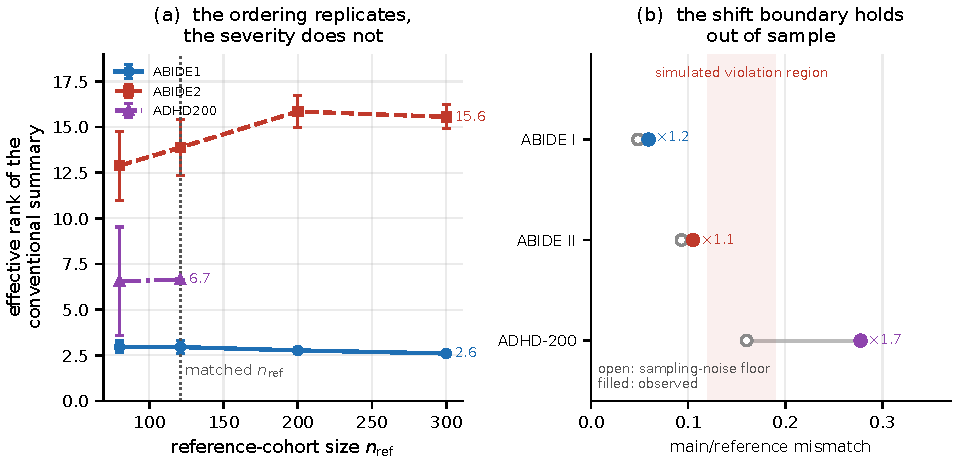
\includegraphics[width=\textwidth]{figs/fig_third.pdf}
\caption{Third-cohort validation: the ordering replicates, the severity does
not. (a) Effective rank of the conventional summary against matching
reference-cohort size (error bars, one standard deviation over draws); at
$n_{\mathrm{ref}}=121$ the same summary spans $2.95$ (ABIDE~I) to $13.88$
(ABIDE~II), so the ordering of summary definitions replicates while their
severity does not. (b) Measured main/reference mismatch (filled dot) against
the sampling-noise floor obtained by randomly splitting each cohort into two
groups of the same sizes (open dot); the leader line gives their ratio. ABIDE
I and II sit at $1.2\times$ and $1.1\times$ their floors, so their mismatch is
almost entirely sampling; ADHD-200 sits at $1.7\times$. The panel plots the
observed mismatch against the floor, not their difference: the excess
$0.117$, which is what lands at the lower edge of the simulated violation
region (shaded), is obtained only after the floor is subtracted. Its FDP is
correspondingly violated in the reference-cohort arms.}
\label{fig:third}
\end{figure}

\paragraph{The ordering replicates; the severity does not.}
In ADHD-200, as in both ABIDE cohorts, the conventional meanconn summary has
the lowest effective rank and partial correlation the highest
($6.65$ against $25.98$ for pcresid and $40.20$ for partial). But the
\emph{severity} is cohort-specific: at matched reference-cohort size
($n_{\mathrm{ref}}=121$) the effective rank of the same summary is $2.95$ in
ABIDE~I and $6.65$ in ADHD-200, and $13.88$ in ABIDE~II. That is exactly
what \S\ref{sec:geometry} predicted---the diagnostic is portable, the
constant is not---and it is the reason we recommend reporting the
diagnostic rather than a threshold.

The positive control on ADHD-200 also reproduces the dependence on the
number of true signals ($1.00$ at $k=12$ against $0.24$--$0.30$ at $k=3$,
at conditional $|t|=6$), so the third cohort does not distinguish the
mechanisms we identify.

\paragraph{The cohort-shift boundary is confirmed prospectively.}
The third cohort does provide an out-of-sample test of
\S\ref{sec:shift}. ADHD-200 has nine sites whose protocols differ
substantially, and its reference cohort is smaller by a factor of $3.2$
($n_{\mathrm{ref}}=121$ against $393$). Its measured main/reference mismatch
is $0.278$, far beyond the simulated violation boundary of
$0.12$--$0.19$ (Figure~\ref{fig:third}b places it against the sampling-noise
floors of all three cohorts), and its FDP behaviour follows: on the injected
control the
reference-cohort arms exceed the nominal level (FDP $0.22$--$0.29$ across
configurations), whereas the arm whose $\hat\Sigma$ comes from the main
cohort itself---which is not a valid model-X procedure, but has no mismatch
to get wrong---stays inside it ($0.16$--$0.18$). The contrast is what
localises the failure to the mismatch between the two distributions, rather
than to something particular about ADHD-200. In both ABIDE cohorts, whose
mismatch is inside the safe region, the reference arms were controlled.

One caution is required, and it is the same caution that applies to any
such comparison. A mismatch measured between two sample correlation
matrices contains sampling noise as well as any genuine distributional
difference, and tiny reference cohorts inflate it mechanically. We
therefore measured the noise floor directly, by randomly splitting each
cohort into two groups of the same sizes---so that the two groups differ
only by sampling---and repeated this twelve times. On that scale ABIDE~I and
ABIDE~II sit at $1.2\times$ and $1.1\times$ their noise floors, so their
measured mismatch is almost entirely sampling; ADHD-200 sits at $1.7\times$,
and the excess that remains after its own floor is subtracted, $0.117$, lands
at the lower edge of the simulated boundary.
Figure~\ref{fig:third}b plots the observed mismatch against the floor, not
this difference. The distinction matters because the two sources have different
consequences---a biased $\hat\Sigma$ is anti-conservative, whereas a merely
noisy one is conservative \citep{candes2018panning}---so a practitioner
comparing mismatches should subtract the noise floor before comparing
against the boundary.

\section{Discussion}
\label{sec:discussion}

The standard account of reference-cohort knockoffs in neuroimaging is that
the estimated covariance is too degenerate to build useful knockoffs from.
We set out to quantify that account and found that it survives as a
description of the spectrum but fails as an explanation of the outcome. The
degeneracy is real; it costs about fourteen percentage points of power; it
does not make the procedure return nothing. We then tested the obvious
alternatives---six constructions, a method that never inverts $\Sigma$, a
cross-environment consistency filter, and a continuous family of
reparameterisations---and all of them fail at the same place. What remains
is the feature geometry, and there the evidence is unambiguous: the
conventional ROI summary is a row mean of a correlation matrix, hence a
proxy for its first principal component, and that is what determines
everything downstream.

\paragraph{The dominant choice is the one made first.}
Our meanconn features have effective rank $2.56$ out of $113$ because a row
mean of a correlation matrix is a proxy for its first principal component
(median $R^2$ of a single feature on PC1: $0.677$). Partial correlation
raises that to $71.6$, and the increase is not an artefact of regularisation:
with no shrinkage at all the effective rank is $59.8$, and across shrinkage
strengths from $0$ to $0.5$ it never falls below $53$. The four standard
summaries agree at median $r\le0.26$ per ROI, every ROI below $0.5$---less
agreement, on the same subjects and the same atlas, than the two
preprocessing pipelines. A literature that reports which parcellation, which
motion threshold and which statistical method was used, but not which ROI
summary, is omitting the choice that moves the features furthest.

\paragraph{The reference cohort is a secondary constraint.}
Three independent manipulations agree that reference-cohort size is not what
decides whether an analysis works, though it is not free either, as a
comparison across arm strengths rather than a single row makes clear. Using the real covariance as ground
truth gives power $0.859$. Reference-cohort size from $100$ subjects to the
full $393$ buys at most nine points of per-signal power, and only at moderate
signal: at conditional $|t|=3$ and $k=12$ the increase is $0.590$ to $0.676$,
narrowing to five points at $|t|=6$, and the sign is the one theory expects
from a noisier $\hat\Sigma$ \citep{candes2018panning}. Cohort distribution
shift at the level actually observed between ABIDE's cohorts \emph{raises}
power. And a method built to avoid $\Sigma^{-1}$ entirely fails at the same
place, for the same reason. Against the effect of the number of true
signals---$0.97$ at $k=12$ against $0.20$ at $k=3$---these are second order.
This is a negative result about a widely assumed bottleneck, and its
practical consequence is one of degree: enlarging a reference cohort buys a
few points of power, while measuring whether the features are usable decides
whether the analysis can work at all.

\paragraph{Two failure modes survive, and both are silent.}
Cohort shift destroys FDP calibration while inflating apparent power
(\S\ref{sec:shift}), which is the direction that looks like success. The
penalty constant of the feature statistic must satisfy a power condition and
a solver-convergence condition simultaneously, and the software reports
neither (\S\ref{sec:penalty}). Both belong to a family that the
matrix-power experiment makes vivid: operations that increase apparent
signal while degrading calibration, whose effect on the numbers a user
actually sees is an improvement. The general lesson is not specific to
knockoffs. Any procedure whose error control is verified through an
internally computed estimate needs that estimate to be validated under the
manipulations the user is free to perform; the aggregating failure of
\S\ref{sec:retained} is the same lesson in a harder form, where the
procedure began reporting discoveries that did not exist.

\paragraph{What a practitioner should do.}
\begin{enumerate}[leftmargin=1.7em,itemsep=3pt]
  \item \textbf{Report the ROI summary's spectrum before any selection.}
  Effective rank, $\ld$ and the first-component share are computable from
  the reference cohort alone, with no pilot and no knockoff draw. On our
  data the conventional summary gives $2.56$ of $113$ with PC1 at $62\%$;
  partial correlation gives $71.6$. A low effective rank means the features
  are close to one number, and no downstream method we tested rescues that.
  \item \textbf{Report which ROI summary was used, and consider more than
  one.} The four standard summaries are almost mutually uncorrelated per
  ROI. Where the summaries disagree, the disagreement is the finding.
  \item \textbf{Do not assume the conventional neuroimaging remedy
  applies.} Global-signal regression helped one pipeline, did nothing for
  another, and reduced the effective rank on ABIDE~II. Removing the leading
  principal components worked everywhere we tried it.
  \item \textbf{Do not expect a larger reference cohort to rescue the
  analysis.} It buys a few points of per-signal power at moderate signal
  ($0.590$ at $100$ reference subjects against $0.676$ at $393$, both at
  $|t|=3$, $k=12$) and fewer at strong signal; that is worth having, but it
  is an order of magnitude smaller than the effect of how many coordinates
  are truly non-null.
  \item \textbf{Report selections as distributions over draws, never as a
  single run.} In our data $35.5\%$ of draws return nonempty selections, and
  a single draw would have justified the opposite conclusion.
  \item \textbf{Validate the penalty constant on both axes before
  interpreting anything.} Check that a signal of known strength survives it
  and that the solver converges; report the convergence rate. The value we
  used originally failed the first test silently.
  \item \textbf{Aggregate with $e$-values, never by averaging the
  statistics.} Averaging the $W$-vectors and thresholding manufactures
  discoveries under a global null.
  \item \textbf{Check that cohort mismatch is inside the safe region.}
  Measure the RMS difference between the reference and main cohort
  correlation matrices. In our simulation FDP control is lost somewhere
  between mismatch $0.12$ and $0.19$; the observed ABIDE~I value is
  $0.0593$.
\end{enumerate}

\paragraph{Relation to prior work.}
Our findings are consistent with the existing robustness theory and give it
an empirical boundary. \citet{barber2020robust} bound the FDR inflation
under a misspecified $F_X$ by a divergence measure; \S\ref{sec:shift}
traces that bound empirically and locates where it is crossed.
\citet{huang2020relaxing} establish that exact control survives an
estimated parametric family but are explicit that the choice of tuning
parameters, including $s$, and the resulting power--robustness tradeoff are
open; our results suggest the more consequential tuning parameter in
practice is not $s$ but the feature statistic's penalty. The construction
literature's motivating pathology---reconstructability minimisation
addressing the rank deficiency of the standard SDP solution when
$\ld(\Sigma)\le0.5$ \citep{spector2022powerful}---is a property of
\emph{knowing} $\Sigma$: estimating it by any shrinkage estimator, from any
sample size, moves $s$ off the constraint boundary. Here the same rank
deficiency reappears from the opposite direction, as a ceiling on what any
construction can achieve when the features themselves are nearly collinear.
On the validity side, our cohort-shift result is the imaging analogue of
reference-panel mismatch in knockoff GWAS
\citep{chen2021ldref,kanai2022slalom}, a problem for which no correction
currently exists in that literature either.

\paragraph{Limitations.}
Seven should be stated plainly.

First, both cohorts study autism. ABIDE~I and II are large and
well-preprocessed but heavily analysed resources, and we make no claim about
autism; the regions the procedure reports should be treated as a
demonstration of method behaviour. Whether these findings extend to other
disorders, to non-clinical phenotypes, or to non-imaging high-dimensional
covariates is untested. We did add a third cohort of a different disorder
(\S\ref{sec:third}, ADHD-200), and it replicates the \emph{ordering} of the
summary definitions while showing that their severity is cohort-specific;
but three cohorts, two of them autism, are not a broad sample, and the
effective ranks we report for the conventional summary span a factor of $4.7$
across them. The diagnostic is what we claim generalises, not any number in
our tables. A fourth cohort---ideally a non-clinical or non-imaging one---would
test that claim further.

Second, and most importantly, the discovery \emph{sets} are not validated at
any level. On real data we have no ground truth, so we cannot compute a
false discovery proportion; the only error numbers in this paper come from
injected signals and global nulls, where the truth is constructed. We
therefore make no claim that any reported ROI is genuinely associated with
diagnosis. We emphasise this because the failure modes we document are
exactly the ones that produce plausible-looking output, and a positive
result obtained under one configuration should not be assumed to survive
another.

Third, the effective-rank severity is partly a property of our summary
definition rather than of functional connectomes in general. That is the
paper's subject, but the constant is not portable: a reader whose ROI
summaries are less globally loaded should expect a larger effective rank
and a smaller effect. We have not tested alternative ROI summaries such as
system segregation, tangent-space covariance, or edge-level features, all of
which are plausible alternatives and at least one of which
\citep{faskowitz2020edge,jo2021edge} has been shown to outperform nodal
summaries for individual identification. Graphical-lasso precision is
preferred to shrinkage-based partial correlation by the largest benchmark in
this area \citep{peterson2023regularized}; we used the latter and report the
unregularised effective rank as a check, but we did not compare the two
directly.

Fourth, our simulations use Gaussian covariates and a linear response. The
mechanisms we identify are properties of the construction, the covariance
estimate and the feature geometry, but their quantitative constants may
differ for other designs. The real response is binary and the statistic is a
linear one; a logistic or nonparametric statistic may behave differently,
though nothing in our argument depends on the statistic's functional form.

Fifth, the multi-environment comparison is underpowered in the configuration
we ran. Its own positive control recovers only $0.100$ of a strong injected
signal, so its empty selection on the real response carries no information
about the data; with larger environments the same control recovers $0.762$
(\S\ref{sec:exhaust}). A version of that test with site-level samples large
enough to have power---by pooling sites or by using a cohort with fewer,
larger sites---remains to be run, and would be the natural way to make the
cross-site question answerable.

Sixth, one alternative statistic could not be evaluated. Masked
likelihood-ratio statistics \citep{spector2024mlr} are penalty-free and
asymptotically optimal and would remove the tuning problem of
\S\ref{sec:penalty} entirely; our implementation did not satisfy the
statistic's defining null-symmetry property and we report no results from
it. Establishing whether it succeeds where the statistics we tested do not
is a natural next step.

Seventh, we do not provide a formal theory for the divergence between reported
and true FDP, nor for the FDP boundary in cohort mismatch, nor for the
dependence of power on the number of non-nulls in this regime. We measure
all three and describe their behaviour; theoretical treatments would be
valuable.

\paragraph{Conclusion.}
The reference cohort is not what limits these analyses, and neither, in the
range we can measure, is the conditioning of the covariance: across $41$
configurations spanning effective rank $2.2$ to $113$, per-signal power never
falls below $0.77$. What the ROI summary statistic decides is the geometry of
the feature space, and that choice---made by convention, measurable before any
analysis is run, and not currently reported---moves the features further than
any downstream decision we could find. What limits power is the number of
true signals; what limits validity is cohort mismatch and the penalty
constant. We recommend reporting all four, and reporting every selection as a
distribution over draws rather than as a single answer.

\section*{Declarations}

\noindent\textbf{Funding.} \quad The authors declare that no funds, grants,
or other support were received during the preparation of this manuscript.

\medskip
\noindent\textbf{Competing interests.} \quad The authors have no relevant
financial or non-financial interests to disclose.

\medskip
\noindent\textbf{Use of large language models.}  \quad
An AI coding assistant (Claude, Anthropic) was used to draft and debug
analysis code, to run and tabulate the experiments reported here, and to
assist with manuscript preparation. All experimental designs, all
scientific claims, and every reported number were directed, checked and
approved by the authors, who take full responsibility for the content.

\medskip
\noindent\textbf{Ethics approval.} \quad Not applicable. This study is a
secondary analysis of three publicly available, de-identified datasets
(ABIDE~I, ABIDE~II and ADHD-200). Ethical approval and informed consent were obtained
by the original data-collecting studies and by the data-sharing initiatives
distributing them; no new data were collected, and no
participant-identifiable information was accessed.

\medskip
\noindent\textbf{Consent to participate / Consent for publication.} \quad
Not applicable (secondary analysis of de-identified public data).

\medskip
\noindent\textbf{Availability of data and material.} \quad ABIDE~I was
obtained from the FCP-INDI public archive
(\url{https://s3.amazonaws.com/fcp-indi}), branches
\texttt{cpac/filt\_noglobal} and \texttt{niak/filt\_noglobal}; these require
neither registration nor a data use agreement. ABIDE~II was obtained from
the same archive (\texttt{Derivatives/DCAN}, no registration required) for
the imaging, and from the NITRC Neuro Bureau file release area
(\url{https://www.nitrc.org/frs/?group_id=383}) for the composite
phenotypic file, which requires a NITRC account and agreement to the 1000
Functional Connectomes Project terms. ADHD-200
\citep{adhd200consortium2012} was obtained from the Neuro Bureau
ADHD-200 Preprocessed repository \citep{bellec2017adhd200}
(\url{http://fcon_1000.projects.nitrc.org/indi/adhd200/}, no registration
required), which distributes the Athena-preprocessed images and their
quality flags. Derived feature matrices for all three cohorts are deposited
at [repository DOI, to be assigned].

\medskip
\noindent\textbf{Code availability.} \quad All analysis code---feature
construction for all four ROI summaries, the knockoff pipeline, the
boundary, positive-control, cohort-shift, draw-distribution,
construction-comparison, Gaussian-mirror, multi-environment and
matrix-power experiments, and the scripts that generate every figure and
table---is available at \url{[repository DOI, to be assigned]}. Every figure
is accompanied by the exact numbers it draws, as
\texttt{paper/figs/source\_data/<figure>.csv}, alongside the 300\,dpi raster
and vector versions of the figure itself. The archive
includes a provenance record for every result file and a
\texttt{verify\_claims.py} script that registers every numeric claim together
with the result file and cell that supports it, checks each one, and fails
loudly if any cannot be traced. The same script scans the manuscript for
numeric literals that no claim covers.

\medskip
\noindent\textbf{Authors' contributions.} \quad J.L.\ conceived the study,
designed the experiments and implemented the analysis; S.Z.\ and X.J.\
contributed to the experimental design and to the interpretation of the
results. J.L.\ wrote the manuscript with input from all authors. All
authors read and approved the final manuscript.

\medskip
\noindent\textbf{Information Sharing Statement.}  \quad
All analysis code, the derived feature matrices and the complete result
tables are openly available; the archive is referenced under Code
availability above and contains a script that registers every numeric claim
with the specific result file and cell that supports it, and checks them all.
Raw imaging data are not redistributed here, but both source archives are
public and are identified, with their access conditions, in Availability of
data and material.

\medskip
\noindent\textbf{Acknowledgements.} \quad Data used in this study were
obtained from the ABIDE~I, ABIDE~II and ADHD-200 initiatives. We acknowledge
the participating sites, the FCP-INDI team for curating and distributing the
ABIDE resources, the Neuro Bureau for hosting the ABIDE~II phenotypic
release and the ADHD-200 Preprocessed repository, and the ADHD-200 Consortium
for making the sample available. We thank the ADHD-200 data providers and
the Athena preprocessing team, on whose quality flags our subject selection
depends.

\begin{thebibliography}{99}

\bibitem[Barber and Cand\`es(2015)]{barber2015controlling}
Barber, R.~F. and Cand\`es, E.~J. (2015).
Controlling the false discovery rate via knockoffs.
\emph{The Annals of Statistics}, 43(5):2055--2085.

\bibitem[Barber et al.(2020)]{barber2020robust}
Barber, R.~F., Cand\`es, E.~J. and Samworth, R.~J. (2020).
Robust inference with knockoffs.
\emph{The Annals of Statistics}, 48(3):1409--1431.

\bibitem[Bates et al.(2021)]{bates2021metropolized}
Bates, S., Cand\`es, E., Janson, L. and Wang, W. (2021).
Metropolized knockoff sampling.
\emph{Journal of the American Statistical Association}, 116(535):1413--1427.

\bibitem[Benner et al.(2017)]{benner2017finemap}
Benner, C., Havulinna, A.~S., J\"arvelin, M.-R., Salomaa, V., Ripatti, S.,
and Pirinen, M. (2017).
Prospects of fine-mapping trait-associated genomic regions by using summary
statistics from genome-wide association studies.
\emph{The American Journal of Human Genetics}, 101(4):539--551.

\bibitem[Cand\`es et al.(2018)]{candes2018panning}
Cand\`es, E., Fan, Y., Janson, L. and Lv, J. (2018).
Panning for gold: `model-X' knockoffs for high dimensional controlled
variable selection.
\emph{Journal of the Royal Statistical Society: Series B}, 80(3):551--577.

\bibitem[Chen et al.(2021)]{chen2021ldref}
Chen, W., Wu, Y., Zheng, Z., Qi, T., Visscher, P.~M., Zhu, Z. and Yang, J.
(2021).
Improved analyses of GWAS summary statistics by reducing data heterogeneity
and errors.
\emph{Nature Communications}, 12:7117.

\bibitem[Chen et al.(2023)]{chen2023systematic}
Chen, S., Li, Z., Liu, L. and Wen, Y. (2023).
The systematic comparison between Gaussian mirror and model-X knockoff
models.
\emph{Scientific Reports}, 13:5478.

\bibitem[The ADHD-200 Consortium(2012)]{adhd200consortium2012}
The ADHD-200 Consortium (2012).
The ADHD-200 Consortium: a model to advance the translational potential of
neuroimaging in clinical neuroscience.
\emph{Frontiers in Systems Neuroscience}, 6:62.

\bibitem[Bellec et al.(2017)]{bellec2017adhd200}
Bellec, P., Chu, C., Chouinard-Decorte, F., Benhajali, Y., Margulies, D.~S.
and Craddock, R.~C. (2017).
The Neuro Bureau ADHD-200 preprocessed repository.
\emph{NeuroImage}, 144:275--286.

\bibitem[Ciric et al.(2017)]{ciric2017benchmarking}
Ciric, R., Wolf, D.~H., Power, J.~D., Roalf, D.~R., Baum, G.~L., Ruparel,
K., et al. (2017).
Benchmarking of participant-level confound regression strategies for the
control of motion artifact in studies of functional connectivity.
\emph{NeuroImage}, 154:174--187.

\bibitem[Cole et al.(2012)]{cole2012global}
Cole, M.~W., Yarkoni, T., Repov\v{s}, G., Anticevic, A. and Braver, T.~S.
(2012).
Global connectivity of prefrontal cortex predicts cognitive control and
intelligence.
\emph{The Journal of Neuroscience}, 32(26):8988--8999.

\bibitem[Craddock et al.(2012)]{craddock2012whole}
Craddock, R.~C., James, G.~A., Holtzheimer, P.~E., Hu, X.~P. and Mayberg,
H.~S. (2012).
A whole brain fMRI atlas generated via spatially constrained spectral
clustering.
\emph{Human Brain Mapping}, 33(8):1914--1928.

\bibitem[Dezeure et al.(2015)]{dezeure2015high}
Dezeure, R., B\"uhlmann, P., Meier, L. and Meinshausen, N. (2015).
High-dimensional inference: confidence intervals, $p$-values and R-software
hdi.
\emph{Statistical Science}, 30(4):533--558.

\bibitem[Di Martino et al.(2014)]{dimartino2014autism}
Di Martino, A., Yan, C.-G., Li, Q., Denio, E., Castellanos, F.~X., Alaerts,
K., et al. (2014).
The autism brain imaging data exchange: towards a large-scale evaluation of
the intrinsic brain architecture in autism.
\emph{Molecular Psychiatry}, 19(6):659--667.

\bibitem[Di Martino et al.(2017)]{dimartino2017abide2}
Di Martino, A., O'Connor, D., Chen, B., Alaerts, K., Anderson, J.~S.,
Assaf, M., et al. (2017).
Enhancing studies of the connectome in autism using the autism brain imaging
data exchange II.
\emph{Scientific Data}, 4:170010.

\bibitem[Eklund et al.(2016)]{eklund2016cluster}
Eklund, A., Nichols, T.~E. and Knutsson, H. (2016).
Cluster failure: why fMRI inferences for spatial extent have inflated
false-positive rates.
\emph{Proceedings of the National Academy of Sciences}, 113(28):7900--7905.

\bibitem[Fan et al.(2025)]{ark2025}
Fan, Y., Gao, L. and Lv, J. (2025).
ARK: robust knockoffs inference with coupling.
\emph{The Annals of Statistics}, 53(2):749--773.

\bibitem[Fan et al.(2020)]{fan2020rank}
Fan, Y., Demirkaya, E., Li, G. and Lv, J. (2020).
RANK: large-scale inference with graphical nonlinear knockoffs.
\emph{Journal of the American Statistical Association}, 115(529):362--379.

\bibitem[Fan et al.(2026)]{fan2026moments}
Fan, Y., Gao, L., Lv, J. and Xu, X. (2026).
Asymptotic FDR control with model-X knockoffs: is moments matching
sufficient?
\emph{Journal of the American Statistical Association}, in press.

\bibitem[Faskowitz et al.(2020)]{faskowitz2020edge}
Faskowitz, J., Esfahlani, F.~Z., Jo, Y., Sporns, O. and Betzel, R.~F.
(2020).
Edge-centric functional network representations of human cerebral cortex
reveal overlapping community structure.
\emph{Nature Neuroscience}, 23(12):1644--1654.

\bibitem[Gotts et al.(2013)]{gotts2013perils}
Gotts, S.~J., Saad, Z.~S., Jo, H.~J., Wallace, G.~L., Cox, R.~W. and
Martin, A. (2013).
The perils of global signal regression for group comparisons: a case study
of autism spectrum disorders.
\emph{Frontiers in Human Neuroscience}, 7:356.

\bibitem[Huang and Janson(2020)]{huang2020relaxing}
Huang, D. and Janson, L. (2020).
Relaxing the assumptions of knockoffs by conditioning.
\emph{The Annals of Statistics}, 48(5):3021--3042.

\bibitem[Ji et al.(2024)]{ji2024differential}
Ji, J., Hou, Z., He, Y., Liu, L., Xue, F., Chen, H. and Yuan, Z. (2024).
Differential network knockoff filter with application to brain connectivity
analysis.
\emph{Statistics in Medicine}, 43(20):3830--3861.

\bibitem[Jo et al.(2021)]{jo2021edge}
Jo, Y., Esfahlani, F.~Z., Faskowitz, J., Chiem, B., Sporns, O. and Betzel,
R.~F. (2021).
Subject identification using edge-centric functional connectivity.
\emph{NeuroImage}, 238:118204.

\bibitem[Kanai et al.(2022)]{kanai2022slalom}
Kanai, M., Elzur, R., Zhou, W., Bhérer, C., Rasheed, H., et al. (2022).
Meta-analysis fine-mapping is often miscalibrated at single-variant
resolution.
\emph{Cell Genomics}, 2(12):100210.

\bibitem[Ke et al.(2024)]{ke2024power}
Ke, Z.~T., Liu, J.~S. and Ma, Y. (2024).
Power of knockoff: the impact of ranking algorithm, augmented design, and
symmetric statistic.
\emph{Journal of Machine Learning Research}, 25(10):1--67.

\bibitem[Ledoit and Wolf(2004)]{ledoit2004honey}
Ledoit, O. and Wolf, M. (2004).
A well-conditioned estimator for large-dimensional covariance matrices.
\emph{Journal of Multivariate Analysis}, 88(2):365--411.

\bibitem[Li et al.(2022)]{li2022multienv}
Li, S., Sesia, M., Romano, Y., Cand\`es, E. and Sabatti, C. (2022).
Searching for consistent associations with a multi-environment knockoff
filter.
arXiv:2106.04118.

\bibitem[Liu and Rigollet(2019)]{liu2019esd}
Liu, J. and Rigollet, P. (2019).
Power analysis of knockoff filters for correlated designs.
\emph{Advances in Neural Information Processing Systems}, 32.

\bibitem[Liu et al.(2022)]{liu2022fast}
Liu, M., Katsevich, E., Janson, L. and Ramdas, A. (2022).
Fast and powerful conditional randomization testing via distillation.
\emph{Biometrika}, 109(2):277--293.

\bibitem[Marek et al.(2022)]{marek2022reproducible}
Marek, S., Tervo-Clemmens, B., Calabro, F.~J., Montez, D.~F., Kay, B.~P.,
Hatoum, A.~S., et al. (2022).
Reproducible brain-wide association studies require thousands of
individuals.
\emph{Nature}, 603(7902):654--660.

\bibitem[Mohanty et al.(2020)]{mohanty2020rethinking}
Mohanty, R., Sethares, W.~A., Nair, V.~A. and Prabhakaran, V. (2020).
Rethinking measures of functional connectivity via feature extraction.
\emph{Scientific Reports}, 10:1298.

\bibitem[Moujaes et al.(2024)]{moujaes2024ketamine}
Moujaes, F., Ji, J.~L., Rahmani, M., Burt, J.~B., et al. (2024).
Ketamine induces multiple individually distinct whole-brain functional
connectivity signatures.
\emph{eLife}, 13:e84173.

\bibitem[Murphy and Fox(2017)]{murphy2017consensus}
Murphy, K. and Fox, M.~D. (2017).
Towards a consensus regarding global signal regression for resting state
functional connectivity MRI.
\emph{NeuroImage}, 154:169--173.

\bibitem[Nguyen et al.(2020)]{nguyen2020ako}
Nguyen, T.-B., Chevalier, J.-A., Thirion, B. and Arlot, S. (2020).
Aggregation of multiple knockoffs.
\emph{Proceedings of the 37th International Conference on Machine Learning},
3923--3933.

\bibitem[Peterson et al.(2023)]{peterson2023regularized}
Peterson, K.~L., Sanchez-Romero, R., Mill, R.~D. and Cole, M.~W. (2023).
Regularized partial correlation provides reliable functional connectivity
estimates while correcting for widespread confounding.
\emph{bioRxiv}.

\bibitem[Ren and Barber(2024)]{ren2024derandomised}
Ren, Z. and Barber, R.~F. (2024).
Derandomised knockoffs: leveraging e-values for false discovery rate
control.
\emph{Journal of the Royal Statistical Society: Series B}, 86(1):122--154.

\bibitem[Roy and Vetterli(2007)]{roy2007effective}
Roy, O. and Vetterli, M. (2007).
The effective rank: a measure of effective dimensionality.
\emph{15th European Signal Processing Conference (EUSIPCO)}, 606--610.

\bibitem[Saad et al.(2012)]{saad2012trouble}
Saad, Z.~S., Gotts, S.~J., Murphy, K., Chen, G., Jo, H.~J., Martin, A. and
Cox, R.~W. (2012).
Trouble at rest: how correlation patterns and group differences become
distorted after global signal regression.
\emph{Brain Connectivity}, 2(1):25--32.

\bibitem[Spector and Fithian(2024)]{spector2024mlr}
Spector, A. and Fithian, W. (2024).
Asymptotically optimal knockoff statistics via the masked likelihood ratio.
arXiv:2212.08766.

\bibitem[Spector and Janson(2022)]{spector2022powerful}
Spector, A. and Janson, L. (2022).
Powerful knockoffs via minimizing reconstructability.
\emph{The Annals of Statistics}, 50(1):252--276.

\bibitem[Tzourio-Mazoyer et al.(2002)]{tzourio2002automated}
Tzourio-Mazoyer, N., Landeau, B., Papathanassiou, D., Crivello, F., Etard,
O., Delcroix, N., Mazoyer, B. and Joliot, M. (2002).
Automated anatomical labeling of activations in SPM using a macroscopic
anatomical parcellation of the MNI MRI single-subject brain.
\emph{NeuroImage}, 15(1):273--289.

\bibitem[van den Heuvel et al.(2025)]{vandenheuvel2025lnm}
van den Heuvel, M.~P., Libedinsky, I., Quiroz Monnens, S., Repple, J.,
Sommer, I. and Cocchi, L. (2025).
Investigating the methodological foundation of lesion network mapping.
\emph{Nature Neuroscience}.

\bibitem[Wang and Janson(2022)]{wang2022power}
Wang, W. and Janson, L. (2022).
A power analysis of the conditional randomization test and knockoffs.
\emph{Biometrika}, 109(3):631--645.

\bibitem[Wang and Ramdas(2022)]{wang2022ebh}
Wang, R. and Ramdas, A. (2022).
False discovery rate control with e-values.
\emph{Journal of the Royal Statistical Society: Series B}, 84(3):822--852.

\bibitem[Weinstein et al.(2022)]{weinstein2023power}
Weinstein, A., Su, W.~J., Bogdan, M., Barber, R.~F. and Cand\`es, E.~J.
(2022).
A power analysis for model-X knockoffs with $\ell_p$-regularized
statistics.
arXiv:2007.15346.

\bibitem[Xing et al.(2023)]{xing2023gaussian}
Xing, X., Zhao, Z. and Liu, J.~S. (2023).
Controlling false discovery rate using Gaussian mirrors.
\emph{Journal of the American Statistical Association}, 118(541):222--241.

\bibitem[Zhang(2026)]{zhang2026mirror}
Zhang, X. (2026).
Mirror and knockoff$+$ thresholds under dependence.
arXiv:2607.17084.

\bibitem[Zhao et al.(2025)]{zhao2025tilted}
Zhao, Q., Service, S.~K., Bearden, C.~E., Lopez-Jaramillo, C., Freimer,
N.~B. and Sabatti, C. (2025).
Tilted knockoffs for secondary phenotypes.
arXiv:2508.18548.

\end{thebibliography}

\end{document}
